\documentclass[10pt,twoside, fleqn]{memoir}
%\usepackage{createspace}
%\usepackage[size=pocket,noicc]{createspace}
%\usepackage[paperwidth=4.25in, paperght=6.875in,bindingoffset=.75in]{geometry}
\usepackage[T1]{fontenc}
\usepackage{mathpazo} % USE PALATINO FONT
%\usepackage{newpxtext,newpxmath}
\usepackage[latin1]{inputenc}
%\usepackage[xindy]{imakeidx}
%\usepackage{imakeidx}
\usepackage[nomain,acronym,xindy,toc]{glossaries}
%\usepackage{glossaries} %For acronyms
\usepackage[british]{babel}
%\usepackage{tgtermes}
%\usepackage[framed, numbered, autolinebreaks]{mcode} %MATLAB Snippet code
\usepackage{listings}
\usepackage{graphicx}
\usepackage{glossaries}
\usepackage{hyperref} % HYPERLINKS
\usepackage[font=footnotesize]{caption}
%\usepackage[hidelinks]{hyperref}
%\usepackage{xcolor}

\usepackage{subcaption}
\usepackage{pdflscape} %Landscape pages
\usepackage{pdfpages} %Insert pdf in document
\usepackage{amsmath}
\usepackage{amssymb}
\usepackage{gensymb} %Degree sign
\usepackage{footnote} %Footnotes in tabulars
\usepackage{xcolor,framed,marginnote,blindtext}
\hypersetup{
    colorlinks,
    linkcolor={blue!50!black},
    citecolor={blue!50!black},
    urlcolor={blue!80!black}
}% Get rid of that MySpace feeling in hypelinks...
\usepackage{listings} %Include code
\usepackage{multirow}
\usepackage{datetime}
%\usepackage{svg}

\definecolor{infobackground}{RGB}{217,237,247}
\definecolor{infoforeground}{RGB}{58,135,173}
\definecolor{infoborder}{RGB}{188,232,241}
\usepackage{environ}
\usepackage{tikz} %TO CREATE BLOCK DIAGRAMS
\usetikzlibrary{fit,backgrounds,calc}
%\usepackage{vrsion}
\colorlet{shadecolor}{blue!10}
%\usepackage[fleqn]{amsmath}
\usetikzlibrary{shapes,arrows}
\usetikzlibrary{positioning}

\setcounter{tocdepth}{2} % DEPTH OF TABLE OF CONTENTS; 2= SUBSECTIONS INCLUDED
\setcounter{secnumdepth}{2} % SUBSECTIONS ARE NUMBERED

\usepackage[clockwise, figuresright]{rotating}
\usepackage{longtable}
\usepackage{tabu}

\NewEnviron{alertinfo}[1]
{
    \begin{tikzpicture}
    \node[inner sep=0pt,
          draw=infoborder,
          line width=1.2pt,
          fill=infobackground] (box) {\parbox[t]{.99\textwidth}
        {%
            \begin{minipage}{.15\textwidth}
                \centering\tikz[scale=3]
                \node[scale=1]
                {
                    \includegraphics[scale=0.04]{./Images/Warning.png}
                };
            \end{minipage}%
           \begin{minipage}{.80\textwidth}
                \vskip 10pt
                \textbf{\textcolor{infoforeground}{#1}}\par\smallskip
                \textcolor{infoforeground}{\BODY}
                \par\smallskip
            \end{minipage}\hfill
        }%
    };

    \end{tikzpicture}
}

\newdateformat{monthyeardate}{%
  \monthname[\THEMONTH], \THEYEAR}
  
%\usepackage{mathpazo}
%\usepackage[protrusion=true,expansion=true]{microtype}
%\usepackage{type1cm}
%\usepackage{lettrine}

%\checkandfixthelayout

% See the ``Memoir customise'' template for some common customisations
% Don't forget to read the Memoir manual: memman.pdf

%\title{TITLE OF BOOK}
%\author{NAME OF AUTHOR}
%\date{} % Delete this line to display the current date

%% BEGIN TITLE

\makeatletter
\def\maketitle{%
  \null
  \thispagestyle{empty}%
  \vfill
  \begin{center}\leavevmode
    \normalfont
    {\LARGE\raggedleft \@author\par}%
    \hrulefill\par
    {\huge\raggedright \@title\par}%
    \vskip 1cm
  {\Large \@date\par}%
  \end{center}%
  \vfill
  \null
  \cleardoublepage
  }
\makeatother
\author{Paolo Baesso}
\title{AIDA Trigger logic unit (TLU v1E)}
\date{\today}
\loadglsentries{O:/LatexFiles/Glossary/myGlossary.tex}
%\input{O:/LatexFiles/Glossary/myGlossary.tex}
%\makeglossaries


%%% BEGIN DOCUMENT
\makeindex
\begin{document}

\def\brd{FMC\_TLU\_v1E }
\def\oldbrd{FMC\_TLU\_v1C }

\let\cleardoublepage\clearpage


\maketitle
\frontmatter

\null\vfill
\begin{flushleft}
\textit{Board \brd.}\newline
\newline
Paolo Baesso - \monthname,   \the\year\newline paolo.baesso@bristol.ac.uk
\bigskip

\end{flushleft}
\let\cleardoublepage\clearpage

\newpage
\tableofcontents

\mainmatter
\sloppy

\newenvironment{SpecialPar}
  {\begin{shaded}\noindent}
  {\end{shaded}}



%%% INCLUDE CHAPTERS

%\def\conn{\verb|HDMI1|}
%\def\conn{\verb|HDMI2|}
%\def\conn{\verb|HDMI3|}
%\def\conn{\verb|HDMI4|}
%\include{ch_Introduction}




\chapter{Introduction}\label{ch:introduction}
Congratulations on acquiring an AIDA2020 \gls{tlu}. We hope that the unit will help you to collect lots of useful data during your hardware tests.\\
This manual describes the \gls{tlu} designed for the \href{http://aida2020.web.cern.ch/}{AIDA-2020 project} by David Cussans\footnote{University of Bristol, Particle Physics group} and Paolo Baesso\footnote{University of Bristol, Particle Physics group}.\\
The unit is designed to be used in High Energy Physics beam-tests and provides a simple and flexible interface for fast timing and triggering signals at the AIDA pixel sensor beam-telescope.\\
The current version of the hardware is an evolution of the \href{https://twiki.cern.ch/twiki/bin/view/MimosaTelescope/TLU}{EUDET-TLU} and the \href{https://www.ohwr.org/projects/fmc-mtlu/wiki}{miniTLU} and is shipped in a metal enclosure that includes an \gls{fpga} board, the \gls{tlu} \gls{pcb} and an additional power module: the \gls{fpga} is responsible for all the logic functions of the unit, while the \gls{pcb} contains the clock chip, discriminator and interface blocks needed to communicate with other devices. The power module contains programmable \gls{dac} to power photomultipliers and \gls{led} indicators.\\
The current version of the \gls{pcb} is \brd and is designed to plug onto a carrier \gls{fpga} board like any other \gls{fmc} mezzanine board, although its form factor does not comply with the ANSI-VITA-57-1 standard.\\

\section{Overview}
The AIDA \gls{tlu} provides timing and synchronization signals to test-beam readout hardware.\\
When used for within AIDA-2020 specifications, the hardware generates a low-jitter 40~MHz clock or can accept an external clock reference. The external reference clock frequency is not required to be 40~MHz but other values require a dedicated configuration of the clock circuitry on the board. Similarly, by changing the configuration file it is possible to operate the hardware at different clock frequencies.\\
The \gls{tlu} accepts asynchronous trigger signals from up to six external sources, such as beam-scintillators, and generate synchronous signals (including global trigger or control signals) to send to up to four \gls{dut}. The logic function used to generate the trigger can be defined by the user among all the possible logic combinations of the inputs.\\
Depending on the chosen mode of operation, the \gls{tlu} can accept busy signals or other veto signals from \gls{dut}s and react accordingly, for instance avoiding any further trigger until all the busy signals have been de-asserted.\\
Whenever a global trigger is generated by the unit, a 48-bit coarse time-stamp is attached to it. This time stamp is based on the internal clock. The unit also records a fine-grain time stamp with 780~ps resolution for each signal involved in the trigger decision.\\
The configuration parameters and data are sent and received via the \href{https://www.ohwr.org/projects/ipbus}{IPbus} which provides a simple way to control and communicate TCA-based hardware via the UDP/IP protocol.\\
The \gls{tlu} is shipped with an \gls{fpga} board already programmed with the latest version of the firmware needed to operate the unit. New features and bug fixes are continuously being implemented by the developing team and it is possible to flash the unit with a new firmware as described in section~\ref{ch:flashFPGA}.\\
The unit requires 12~V to operate. Power can be provided using the circular socket located on the back panel. See section~\ref{ch:backpanelintro} for details on compatible connectors.\\
During normal operation the current drawn by the unit is about 1~A.

\section{Front panel}\label{ch:frontpanel}
The front panel of the \gls{tlu} is shown in figure~\ref{fig:frontpanel}; from left to right, the main elements are:
\begin{itemize}
  \item \gls{sfp} cage
  \item 4 \gls{hdmi} connectors for devices under test. Each connector has a \gls{rgb} LED used to indicate the port status (see section~\ref{ch:frontpanelintro}).
  \item 1 LEMO connector for \gls{lvds} clock input/output. This is a 2-pin LEMO series 00 connector\footnote{Part number EPG.00.302.NLN. An example of mating part is LEMO FGG.00.302.CLAD35}. A \gls{rgb} \gls{led} indicator is used to signal whether the port is configured as input or output.
  \item 6 LEMO Trigger inputs. These are standard 1-pin LEMO connectors\footnote{LEMO EPK.00.250.NN. Mates with any LEMO 00.250 connector}. Each input has a \gls{rgb} \gls{led} indicator.
  \item 4 LEMO connectors to provide power to photomultipliers. This is a 4-pin connector with 9-mm diameter\footnote{LEMO part number EXP.0S.304.HLN. Mates with LEMO part FFA.0S.304.CLAC44 or similar.}. For the pin-out see section~\ref{ch:frontpanel}.
  \begin{alertinfo}{Note}
    To reduce the cost of a unit, some modules are not equipped with these connectors and the front panel holes are blanked by a plastic board.\\
    If necessary, it is possible to solder the connectors at a later stage, since all the necessary circuitry is present. This requires disassembling the unit, removing the top cover. See section~\ref{ch:inspection} for details.
  \end{alertinfo}
  \item Green \gls{led} indicators for power (+12 V) and regulators (+5 V and -5 V).
\end{itemize}
\begin{figure}
  \centering
  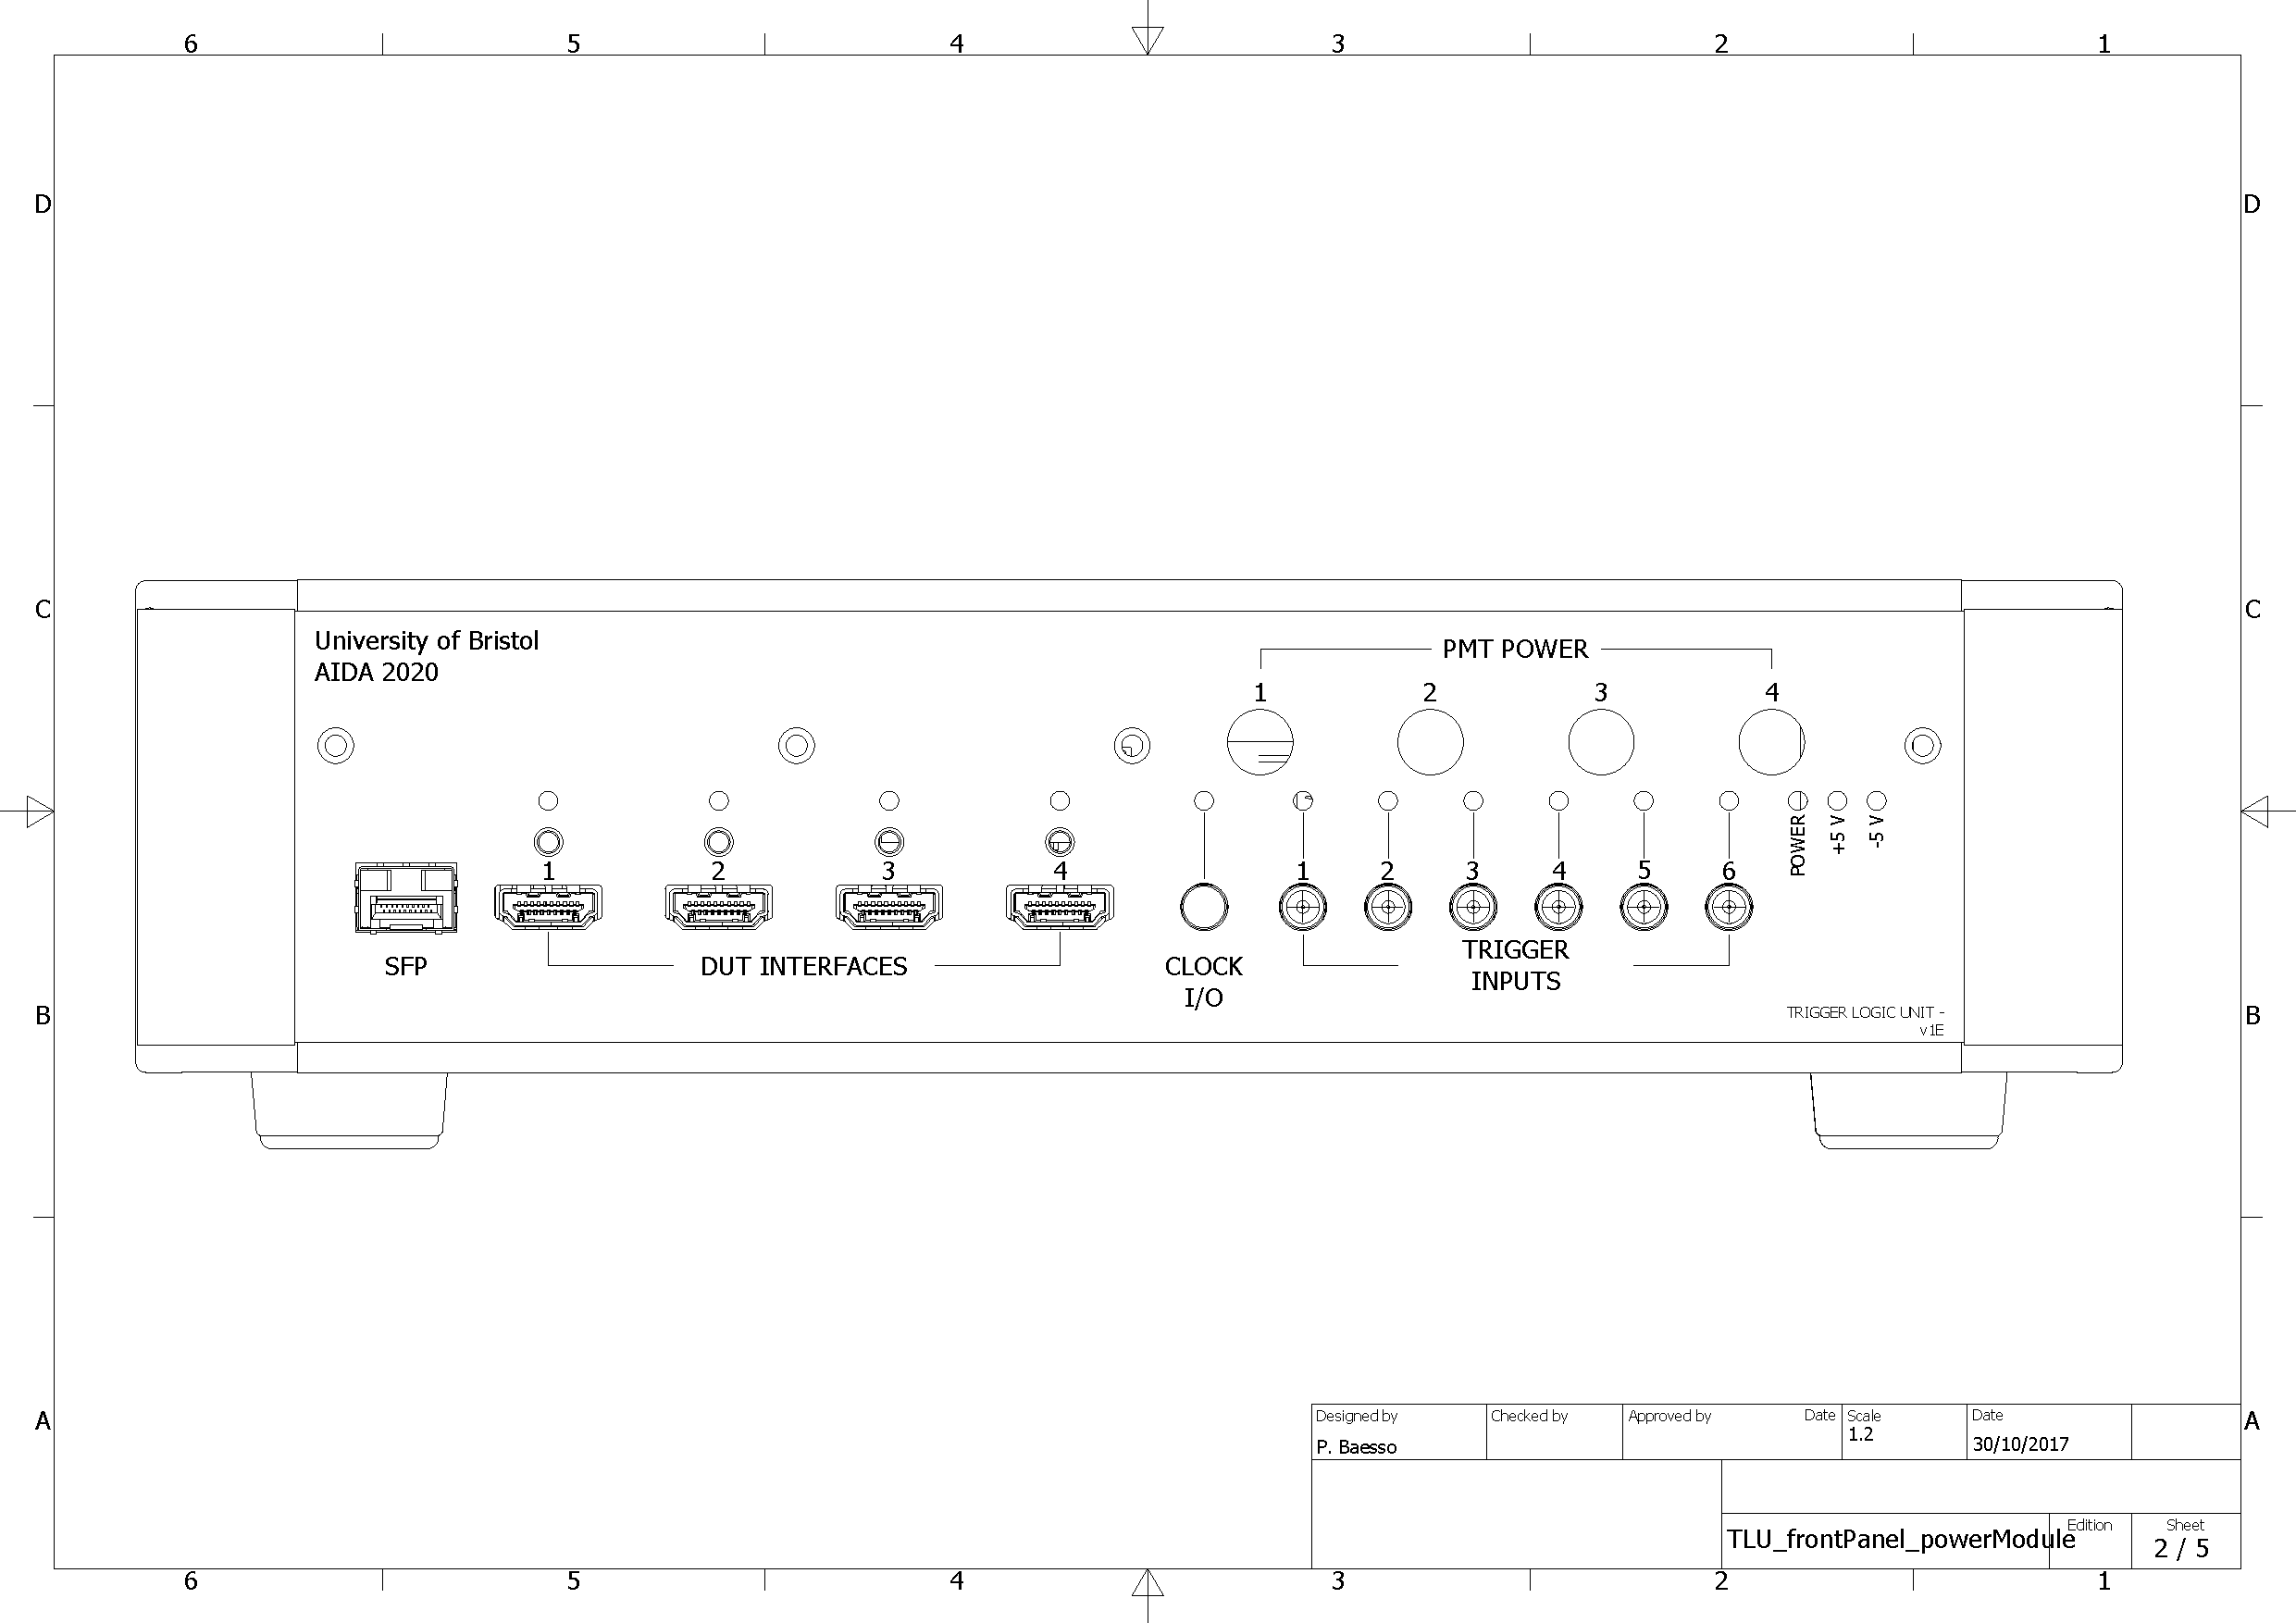
\includegraphics[width=.950\textwidth]{./Images/frontPanel.pdf}
  \caption{View of the TLU front panel.}
  \label{fig:frontpanel}
\end{figure}

\section{Back panel}\label{ch:backpanelintro}
The \gls{tlu} back panel is shown in figure~\ref{fig:backpanel}; from left to right, the main elements are:
\begin{itemize}
  \item RJ45 connector: this is the connector used to communicate with the hardware using IPBus.
  \item \gls{usb}-B port used to flash the internal logic with a new version of the firmware. See section\ref{ch:fpgahardware} for details.
  \begin{alertinfo}{Note}
    This port should be left disconnected if planning to use the self-boot capability of the internal logic. If a cable is detected, the \gls{fpga} will not load the pre-flashed firmware at power-up.
  \end{alertinfo}
  \item \gls{usb}-B port used to communicate with the \gls{fpga} \gls{uart} port.
  \item Power connector\footnote{All TLUs shipped after 17/06/2018 use Switchcraft 721A; mates with a $\phi$~5.5 mm jack with $\phi$~2.5 mm central pin. For instance use Lumberg 1634 02.\\ TLUs shipped before that date use Switchcraft 722A instead, which mates with a $\phi$~5.5 mm jack with $\phi$~2.1 mm central pin. For instance use Lumberg 1633 02. Only 3 units are currently still using the 2.1~mm connector.}. Central pin is +12 V. It is recommended to use a power supply capable of providing at least 1~A.
\end{itemize}
\begin{figure}
  \centering
  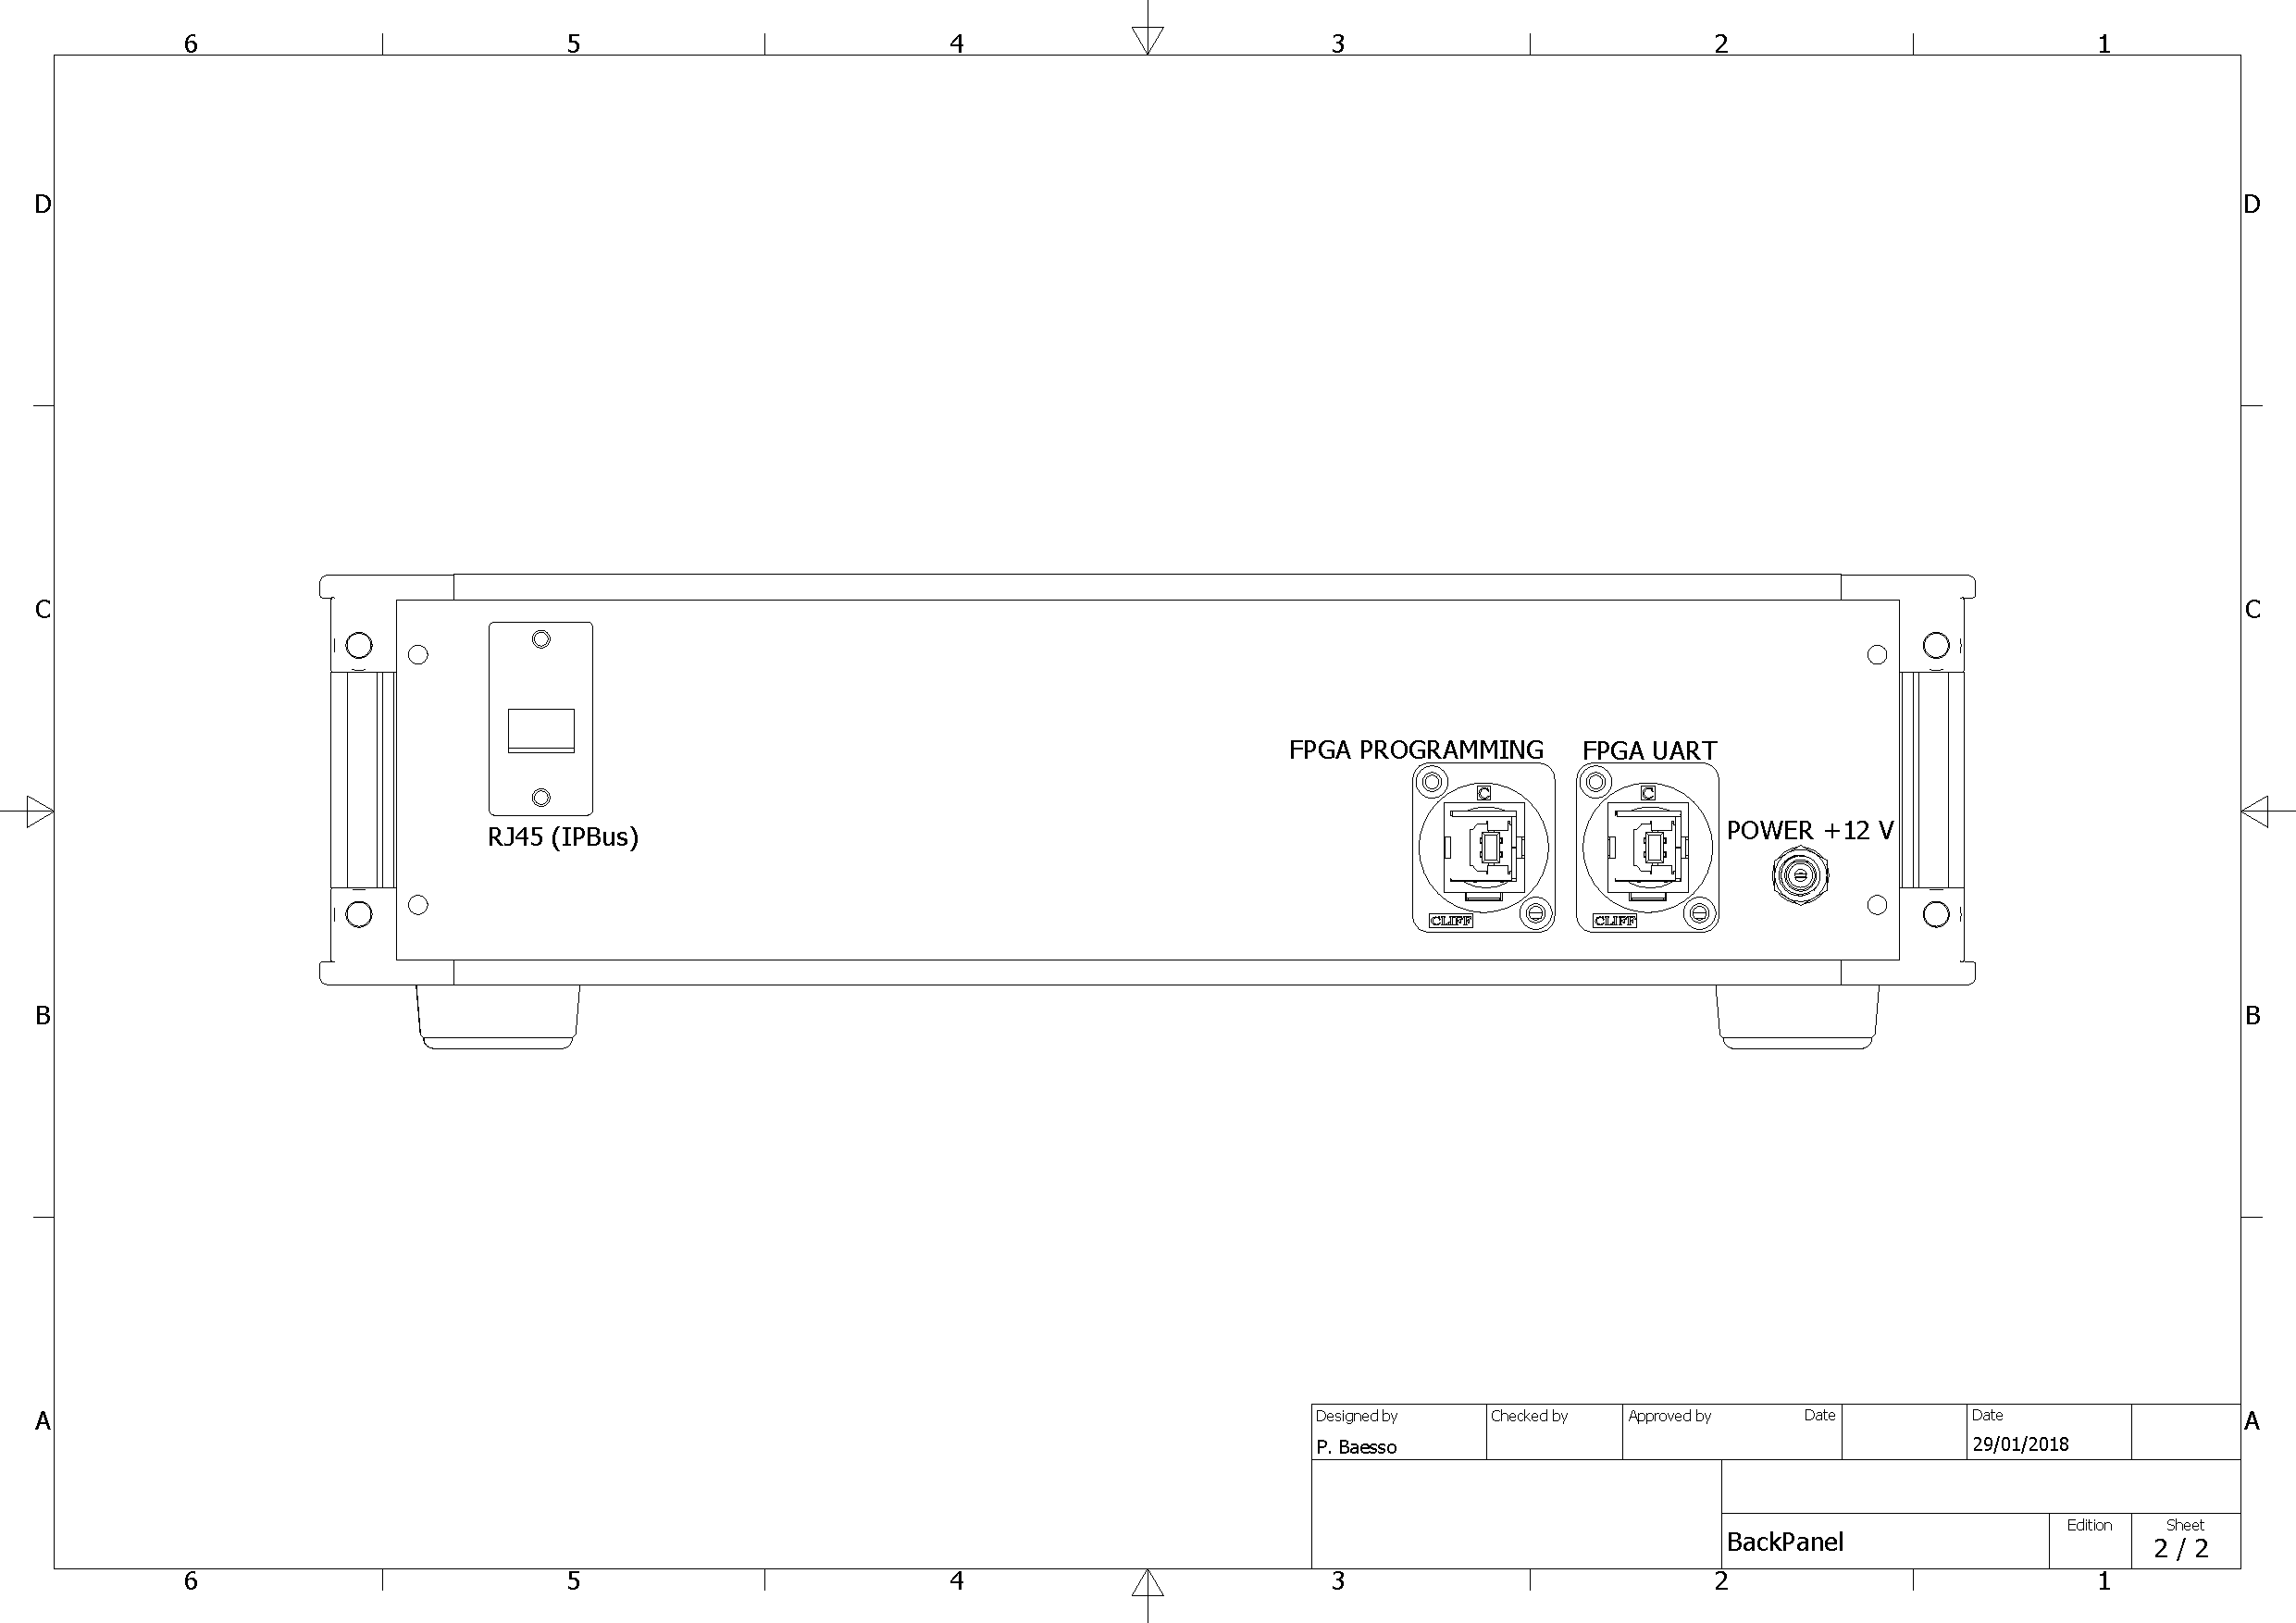
\includegraphics[width=.950\textwidth]{./Images/backPaneldoc.pdf}
  \caption{View of the TLU back panel.}
  \label{fig:backpanel}
\end{figure}
A cooling fan (not shown in figure~\ref{fig:backpanel} is also mounted on the back panel.

\section{Setup}\label{ch:setup}
At the moment of shipping, each \gls{tlu} is pre-configured with the most recent version of the firmware. It is therefore possible to power the unit and start using it almost immediately. The following steps are required to use the unit:
\begin{enumerate}
  \item Ensure no \gls{usb} cable is plugged in the unit
  \item Power the unit using the provided power supply (+12~V) or an equivalent power supply. The pre-configured firmware will automatically load.
  \item Plug an Ethernet cable in the back panel and connect it to the computer used to run the control software. Note that currently the unit uses a pre-defined IP address of 192.168.200.30. In future version of the firmware the address will be configurable.
  \item Use the control software to configure the unit. In particular, after each power up it is necessary to re-configure the clock chip. See chapter~\ref{ch:controlsw} for details on the software and chapter~\ref{ch:clock} for details on the clock chip.
\end{enumerate}

\section{FPGA and firmware}\label{ch:fpgahardware}
The firmware developed at University of Bristol is targeted to work with the Enclustra  AX3 board, which must be plugged onto a PM3 base, also produced by \href{http://www.enclustra.com/en/home/}{Enclustra}. The firmware is written on the \gls{fpga} using a \gls{jtag} interface. Typically a breakout board will be required to connect the Xilinx programming cable to the Enclustra PM3. All these components are included in the \gls{tlu} enclosure so the user can upload a new version of the firmware by simply connecting a \gls{usb}-B cable in the back panel of the unit.\\
At the time of writing this work\footnote{\monthyeardate\today} the AX3 is the only \gls{fpga} for which a firmware has been developed. However, we plan to ship future versions of the \gls{tlu} with a custom made \gls{fpga} designed by Samer Kilani.\\
Each unit is shipped with the latest version of the firmware written onto its boot loader \gls{eeprom}; at power up, the unit will automatically retrieve the firmware from the \gls{eeprom} and program itself.
\begin{alertinfo}{Note}
    If the \gls{fpga} detects a programming cable connected it will not load the firmware from its memory after a power cycle.\\
    It is recommended to leave the \gls{usb} cable disconnected from the back panel unless there is the intention to re-program the firmware.
\end{alertinfo}
The latest version of the firmware can be found on the project github repository (named \href{https://github.com/PaoloGB/firmware_AIDA}{firmware\_AIDA}).\\
The user can decide to configure the unit with a new version of the firmware that will remain active until the \gls{tlu} is powered off (standard programming). It is also possible to write the \gls{eeprom} to replace boot program with a new one (configuration memory programming). Both procedures are described below.
Programming the \gls{fpga} requires the Vivado Lab Tools, available free on the \href{https://www.xilinx.com/support/download.html}{on the Xilinx website}\footnote{https://www.xilinx.com/support/download.html}. Depending on the hardware installed internally, some additional drivers might be required to correctly use the \gls{jtag} cable.\\
At the time of writing, the preferred cable is the Digilent HS2 and the corresponding driver package is ADEPT 2, available on the \href{https://reference.digilentinc.com/reference/software/adept/start}{Digilent website}\footnote{https://reference.digilentinc.com/reference/software/adept/start}.

\subsection{Standard programming}\label{ch:flashFPGA}
Updating the firmware on the \gls{tlu} requires writing a bit stream file to its \gls{fpga}.
This operation is performed using the left \gls{usb} port located on the back panel, labelled \verb"FPGA PROGRAMMING" in figure~\ref{ch:backpanelintro}.\\
Once the Vivado tools have been installed the user should also install the drivers for the programming cable in the enclosure (see previous section for software sources).\\
The bit stream is provided as a \verb".bit" file. They can be found on the firmware \href{https://github.com/PaoloGB/firmware_AIDA/tree/master/bitFiles}{git repository} for the \gls{tlu}\footnote{https://github.com/PaoloGB/firmware\_AIDA/tree/master/bitFiles}.\\
Once these prerequisites are met, the procedure is as follows:
\begin{enumerate}
  \item Open the Vivado tools and select "Hardware manager", figure\ref{fig:hw_open}
  \item Select open target
  \item Identify the cable corresponding to the unit to be written and click open. The cable identifier is generally written on the back panel of the \gls{tlu}. If only one programming cable is connected to the computer, it is possible to use the auto-connect option.\\
      Once done, the Vivado window will be populated, showing the cable and the \gls{fpga} attached to it.
  \item Right click on the \gls{fpga} (typically xc7...) and select \verb"Program device" (see figure~\ref{fig:hw_addMemory})
  \item Locate the \verb".bit" file to be used and program
  \end{enumerate}
\begin{figure}
  \centering
  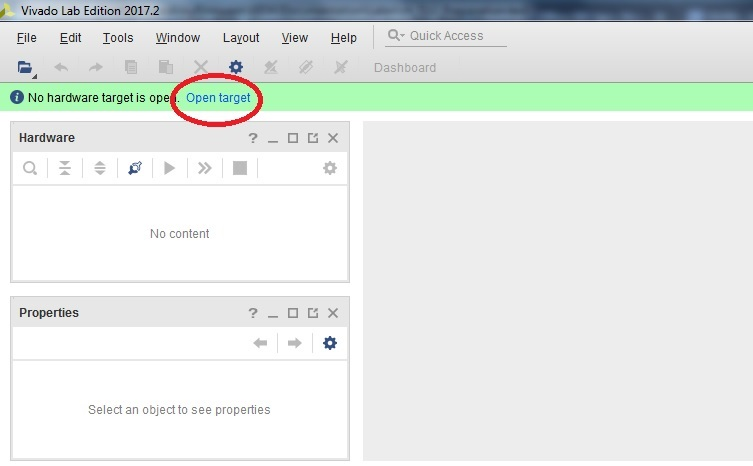
\includegraphics[width=.80\textwidth]{./Images/hw_open.jpg}
  \caption{Vivado interface.}\label{fig:hw_open}
\end{figure}
\begin{figure}
  \centering
  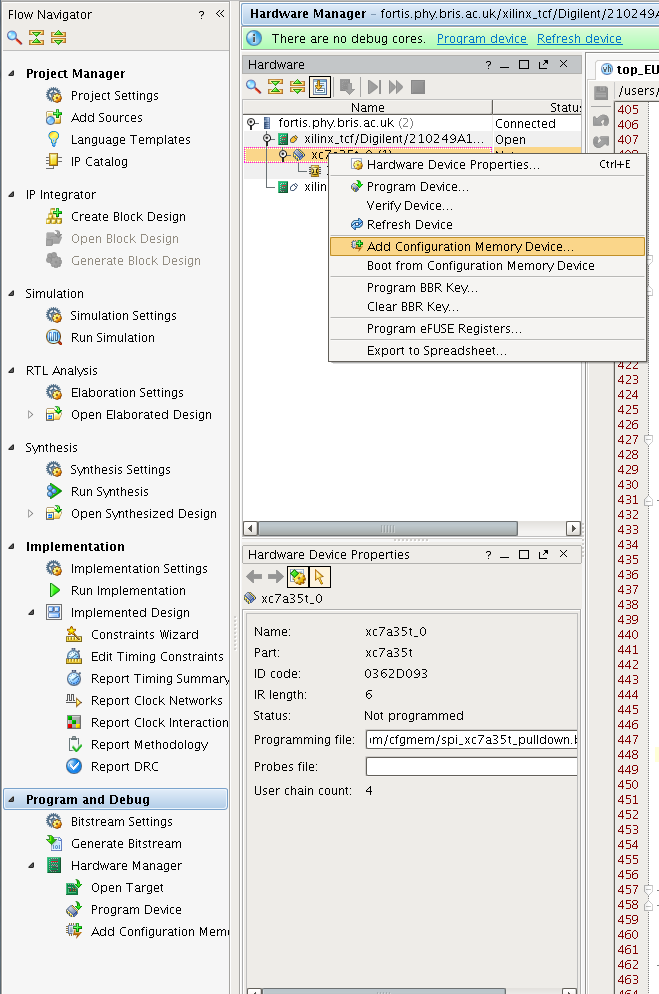
\includegraphics[width=.80\textwidth]{./Images/AddMemory.png}
  \caption{Program interface.}\label{fig:hw_addMemory}
\end{figure}

\subsection{Configuration memory programming}
The procedure to write a permanent program in the \gls{eeprom} is very similar to the one followed to write a bit stream file, with the exception that the user should select \verb"Add configuration memory device" in the options, as shown in figure~\ref{fig:hw_addMemory}.
This will open a new window, shown in figure~\ref{fig:hw_eeprom}, from which it is possible to indicate the file to use (with extension \verb".mcr").
\begin{figure}
  \centering
  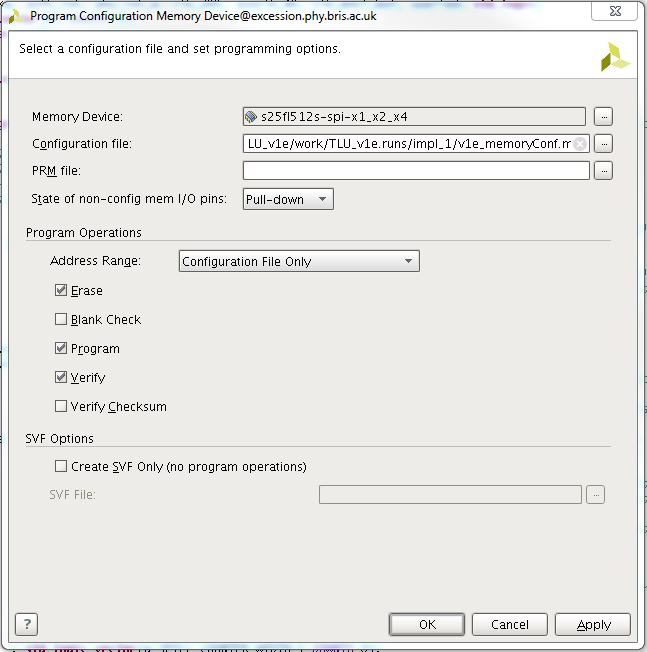
\includegraphics[width=.80\textwidth]{./Images/hw_prog.png}
  \caption{\gls{eeprom} interface. The options shown in the picture are suitable to configure the device correctly.}
  \label{fig:hw_eeprom}
\end{figure}
Make sure that the options are set as shown in figure~\ref{fig:hw_eeprom}.

\section{Inspection}\label{ch:inspection}
At some point someone, somewhere, will want to disassemble the unit to poke at its internal electronics; the top cover of the unit can only slide away when either the front or back frame are removed.
\begin{alertinfo}{Note}
    Simply removing the corner screws on the panels will only allow to remove the plates but not accessing the inside of the unit.
\end{alertinfo}
The frames are held in place by 4 screws hidden behind the corner covers.\\Figure~\ref{fig:dismantle} shows the correct procedure to remove the cover:\\
A) the easiest way to remove the cover is by removing the back frame, rather than the front one.\\
B) Do not remove the corner screws in the plate.\\
C) Remove the two corner covers from the frame. They are only held in place by pressure and can be removed pulling by hand. Once done, remove the 4 Philips screws located behind (green circles).\\
D) unscrew the Philips screw at the bottom of the unit holding the frame in place.\\
E) remove the frame and the back panel. Be careful to not damage the cables connecting the panel to the electronics.\\
F) Slide the top cover away.\\
The same procedure can be repeated with the front frame, if necessary. In this case, the user must also disconnect the front panel from the electronics by removing the countersunk screws connected to the \gls{hdmi} ports and the powermodule.
\begin{figure}
\centering
    \subfloat[A]{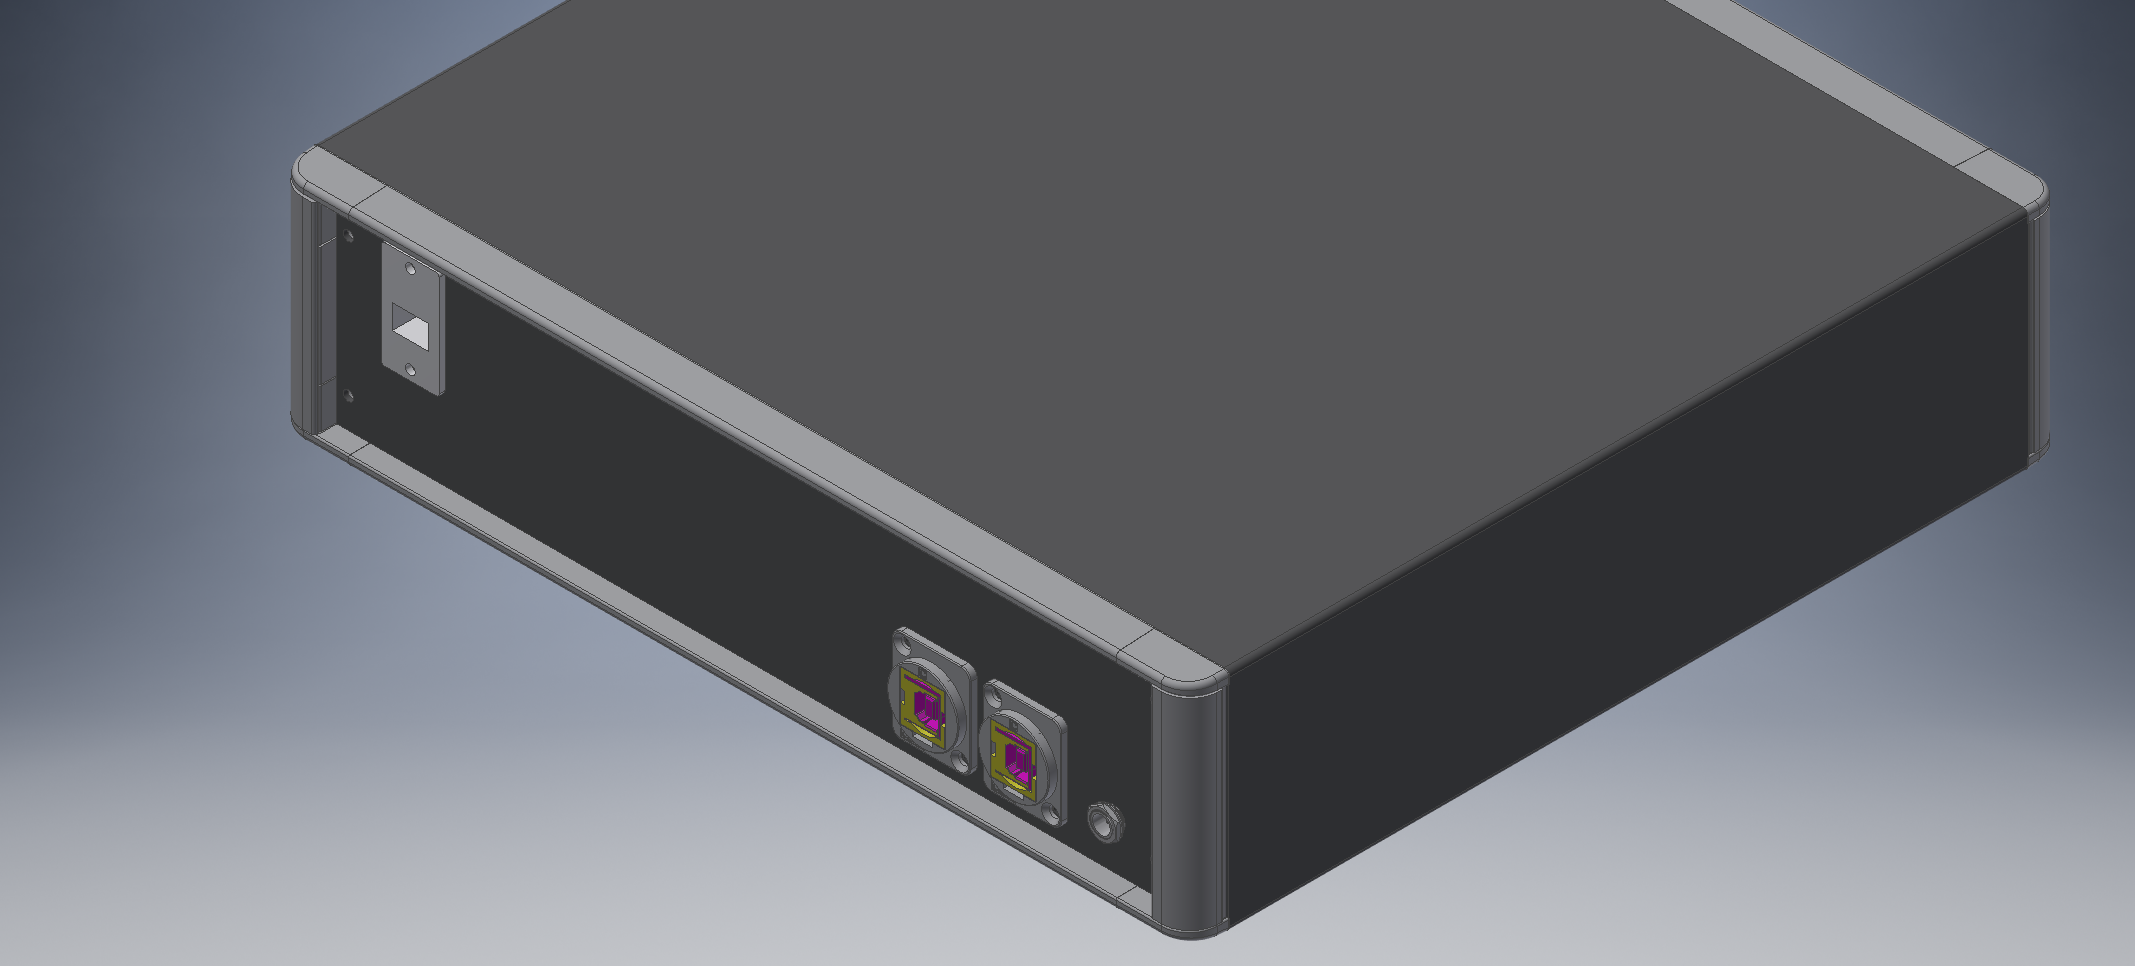
\includegraphics[width=.45\textwidth]{./Images/View1.png}}\hfil
    \subfloat[B]{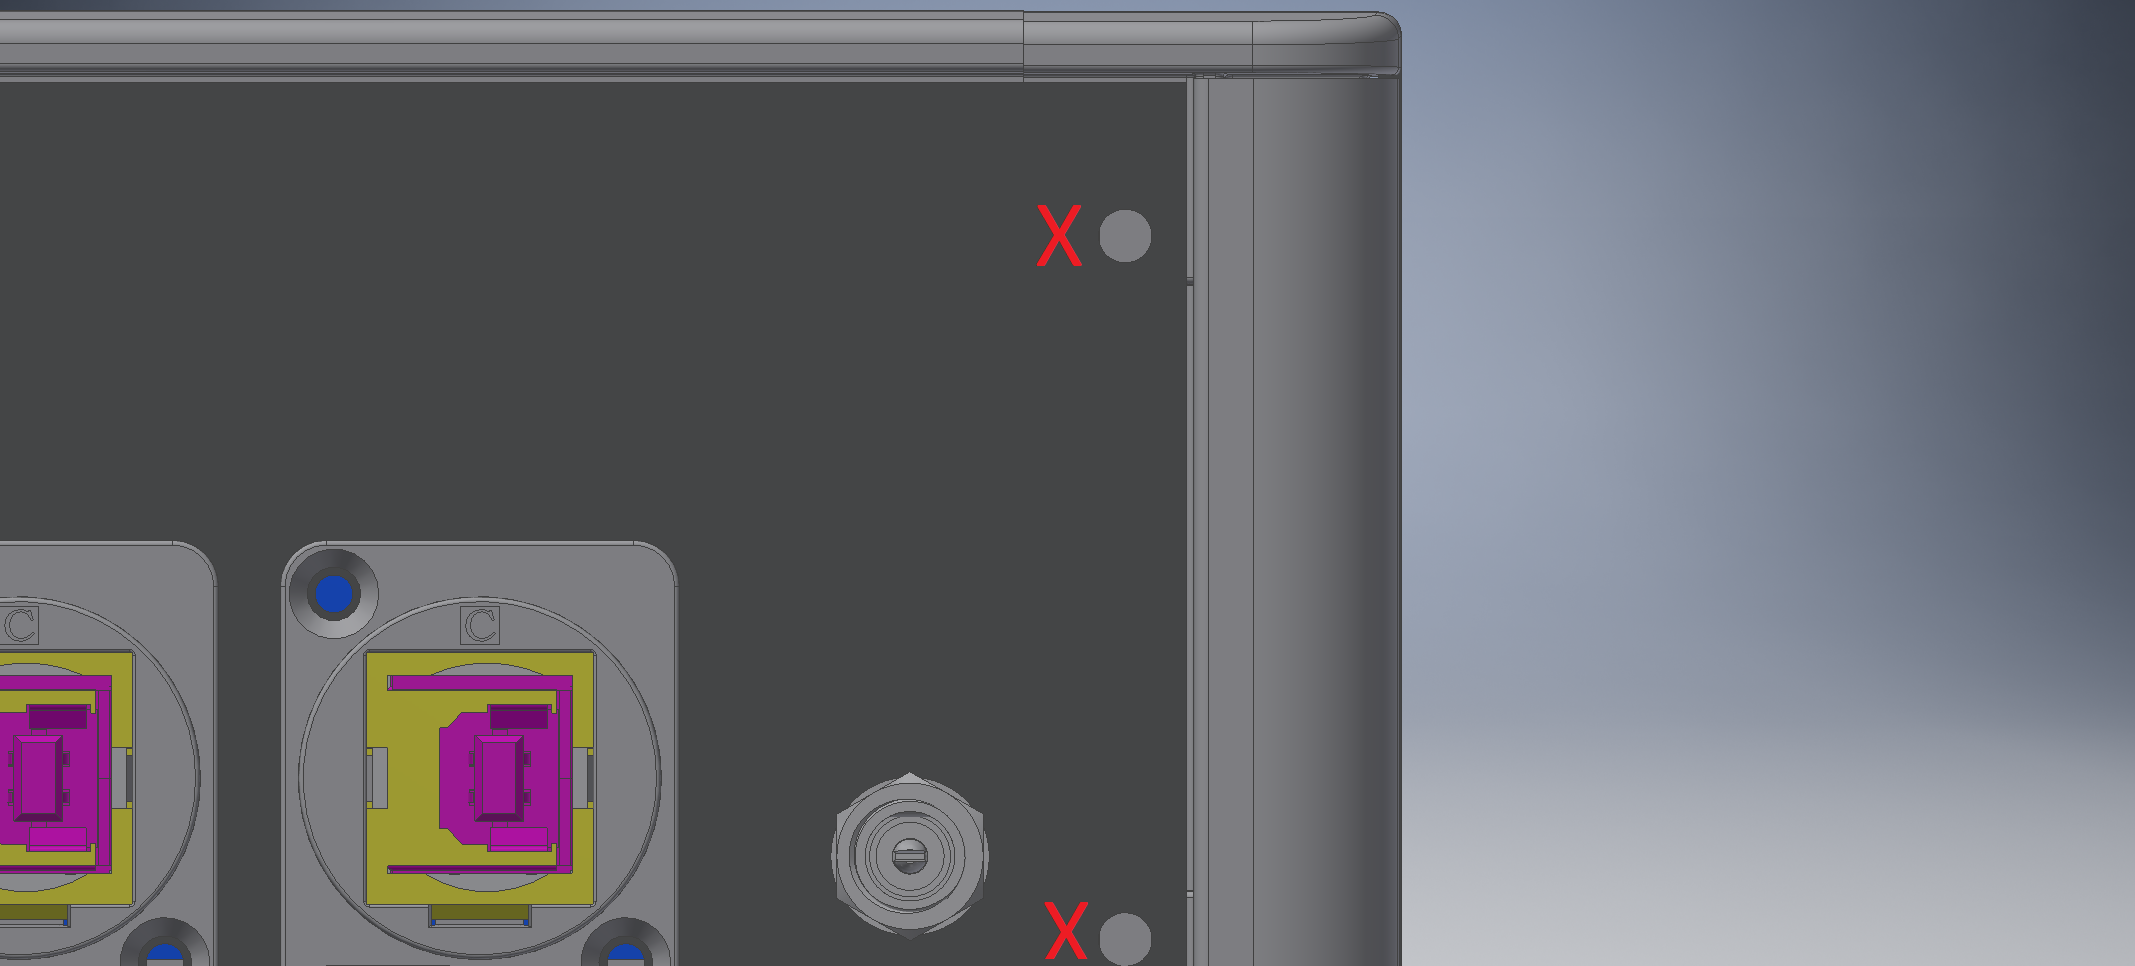
\includegraphics[width=.45\textwidth]{./Images/View6.png}}
    \subfloat[C]{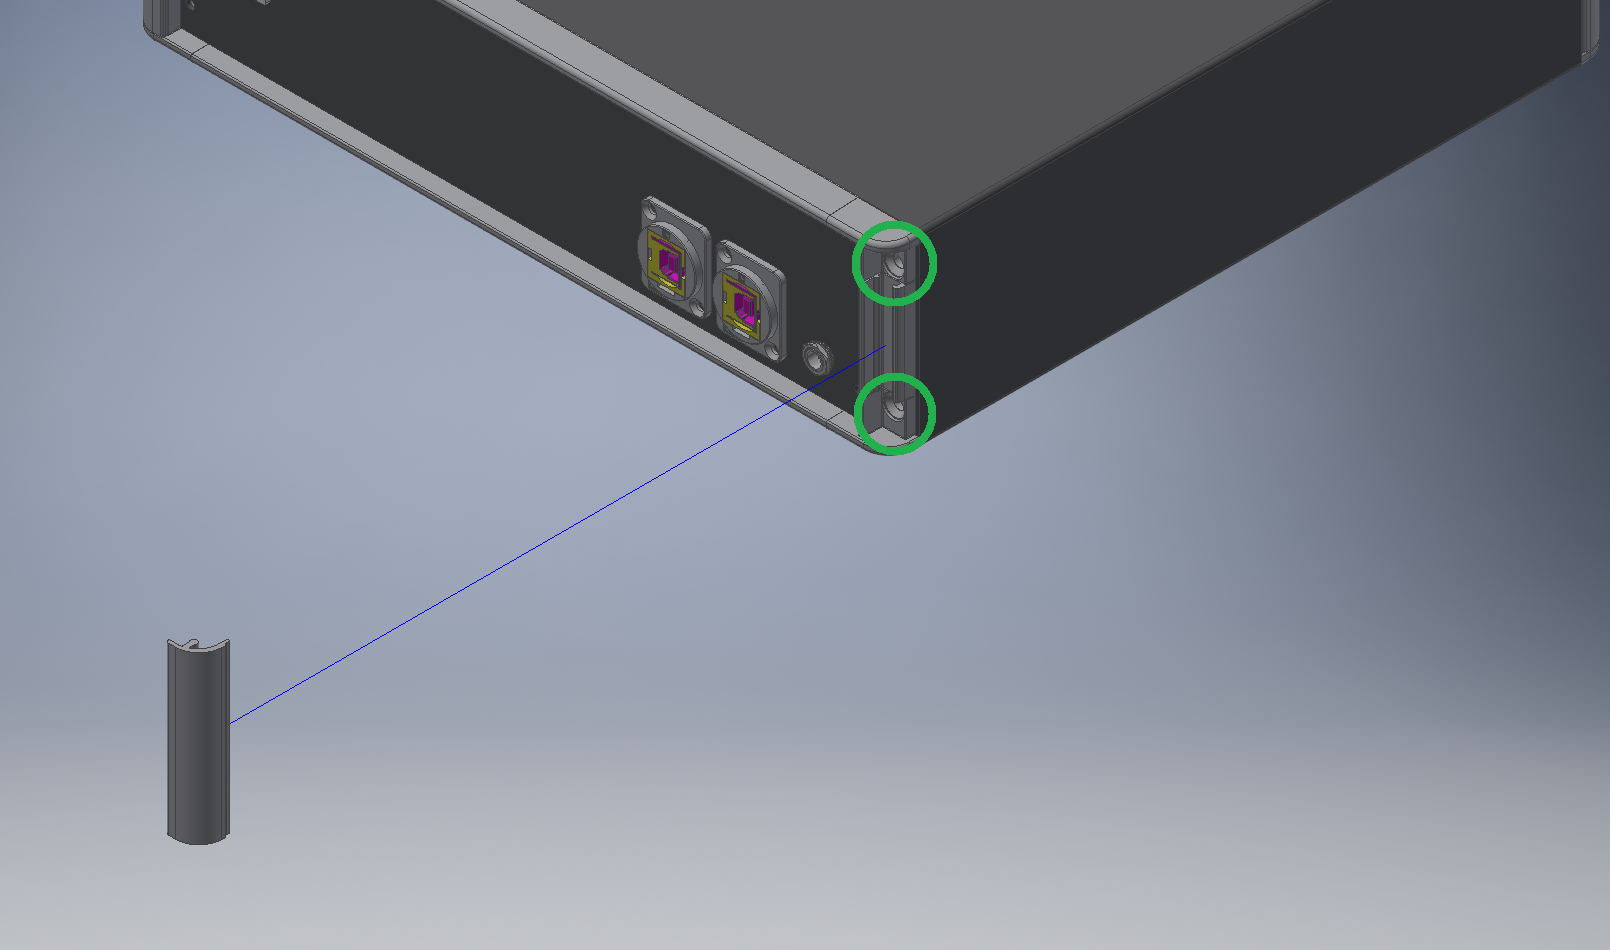
\includegraphics[width=.45\textwidth]{./Images/View2.png}}\hfil
    \subfloat[D]{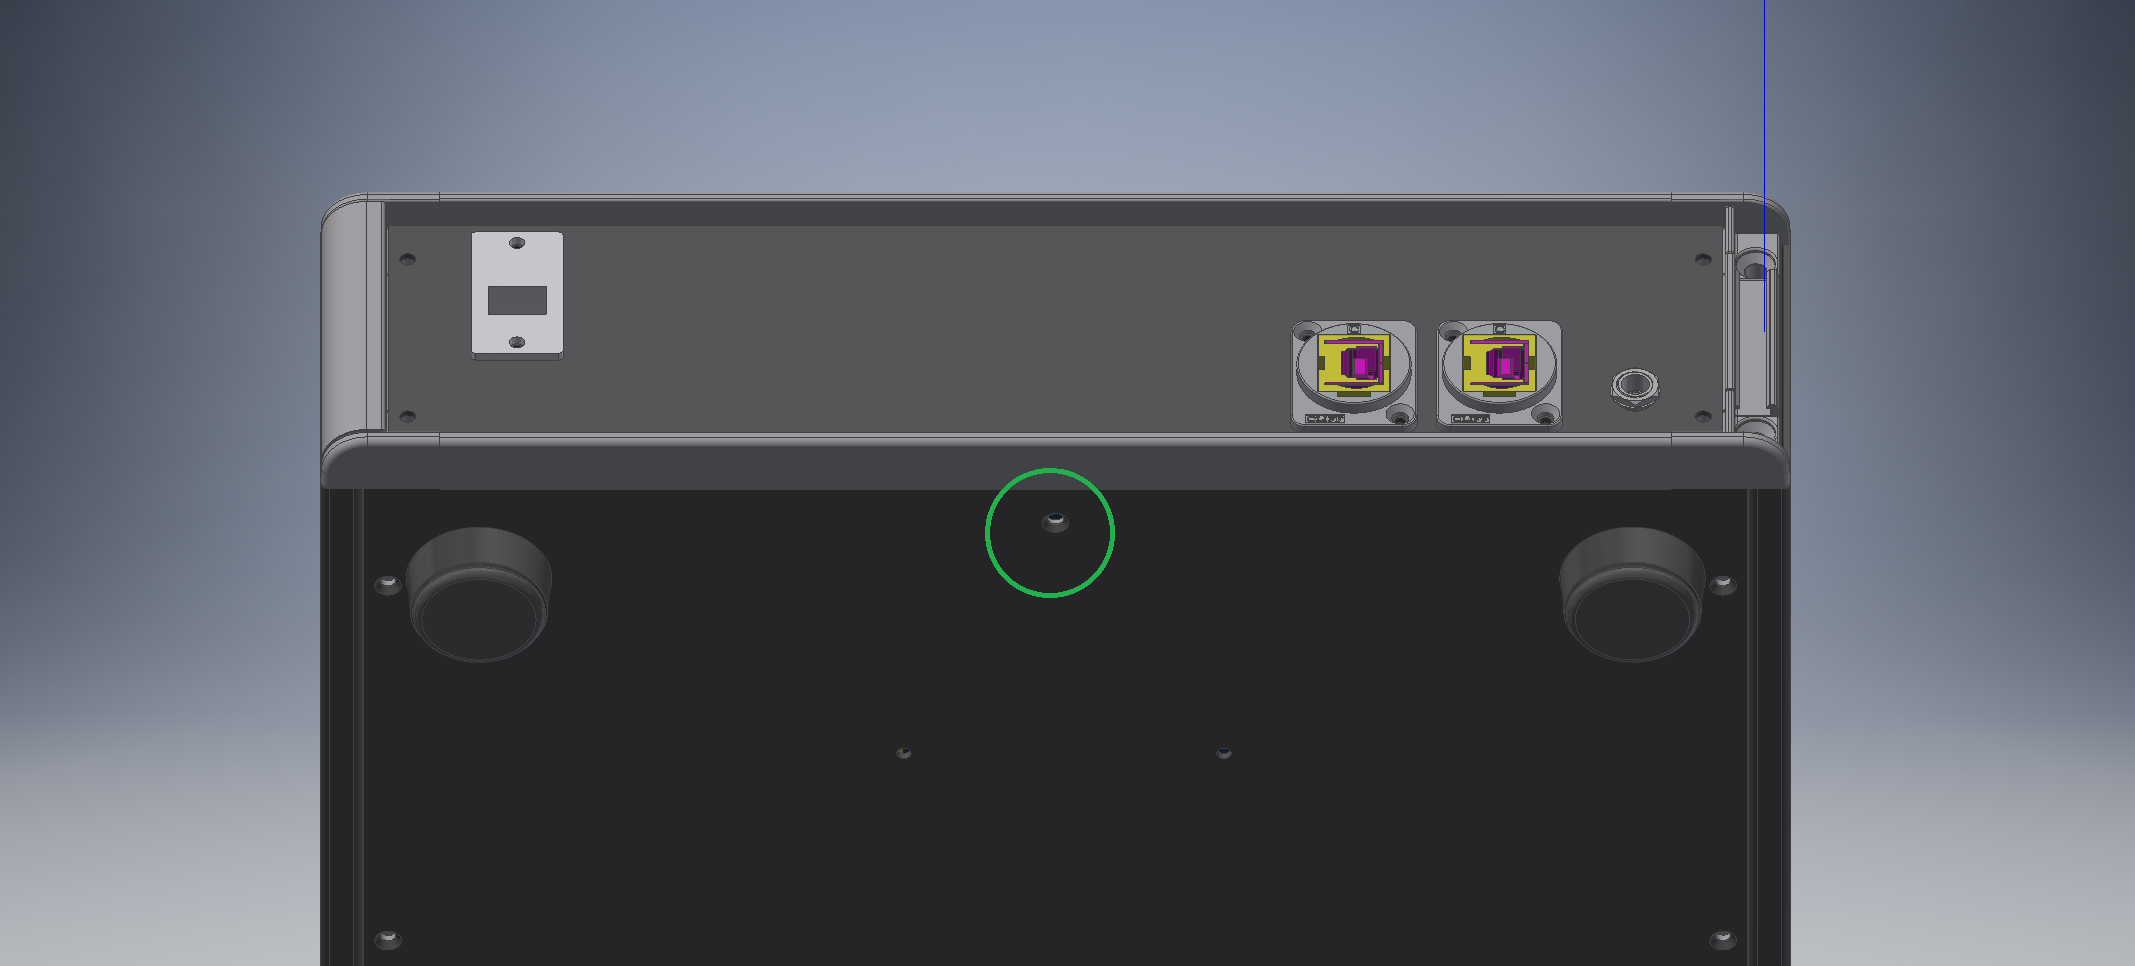
\includegraphics[width=.45\textwidth]{./Images/View3.png}}
    \subfloat[E]{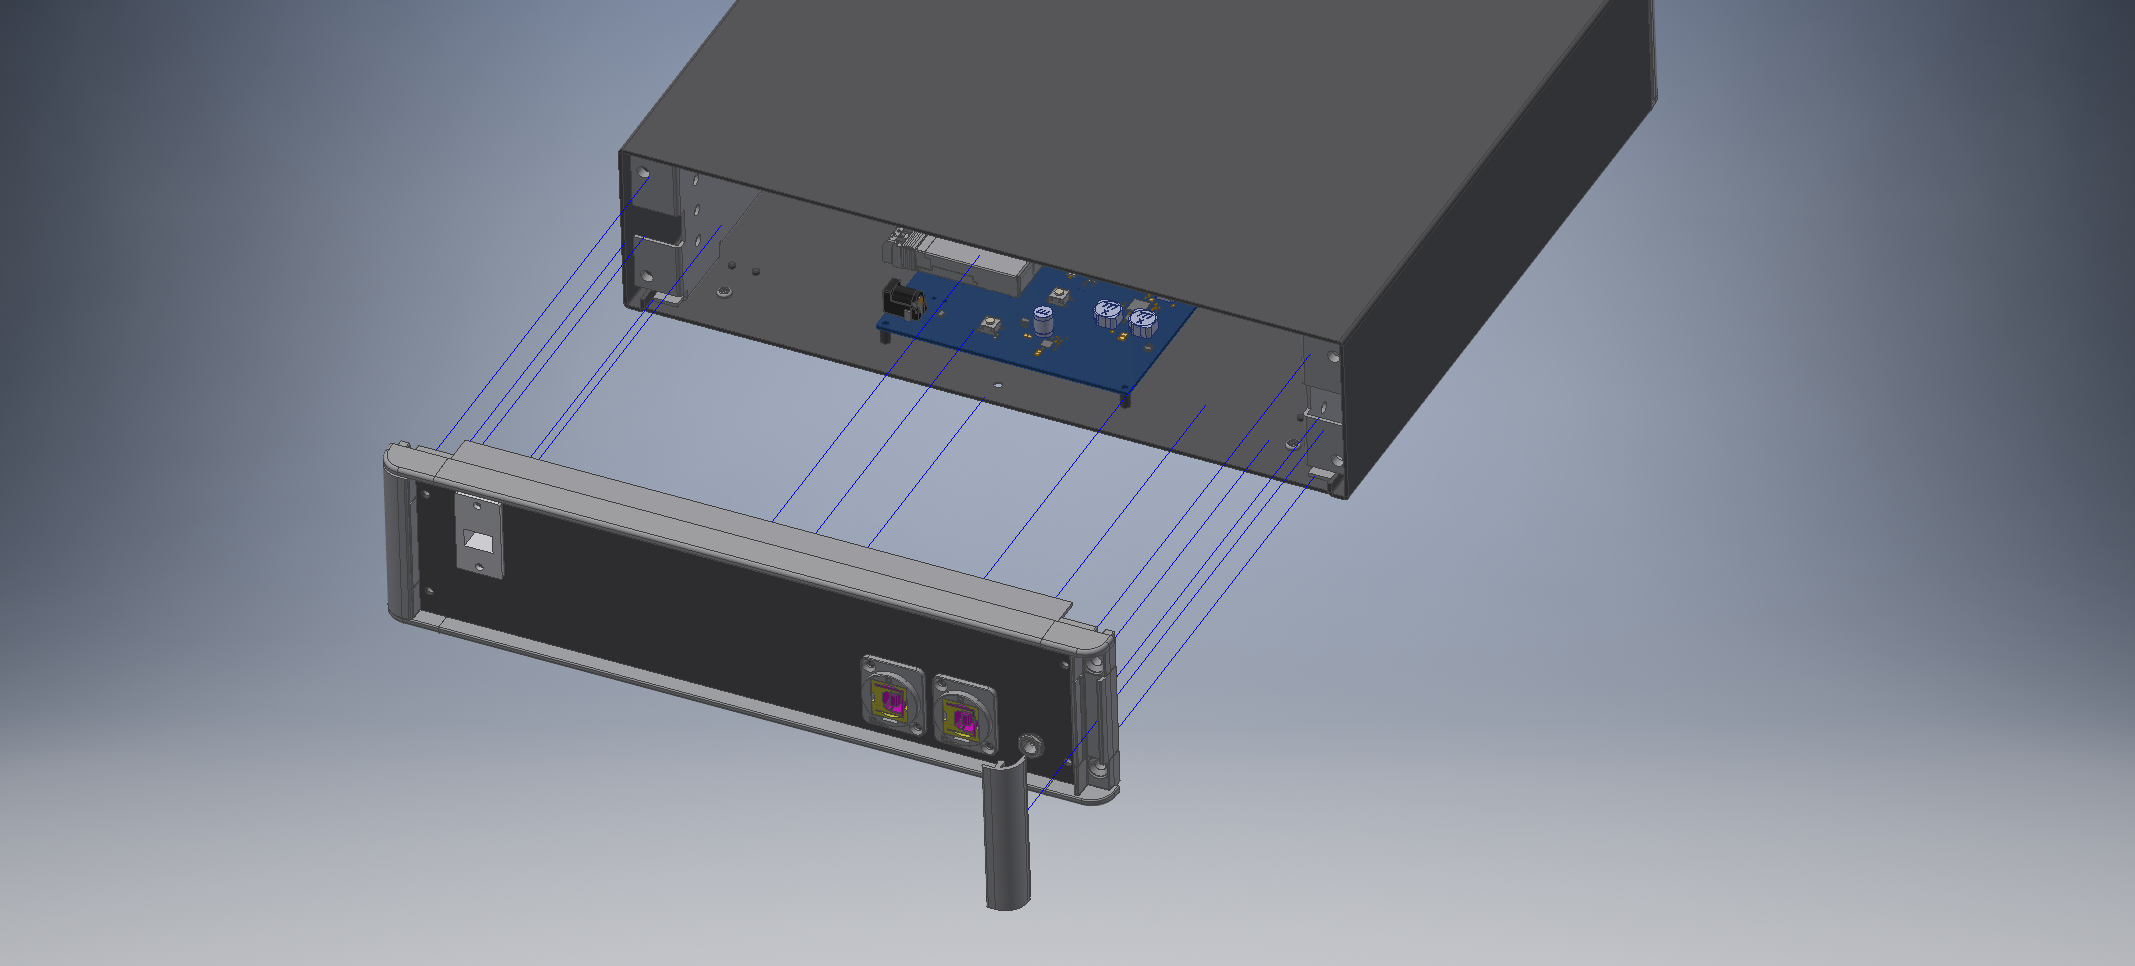
\includegraphics[width=.45\textwidth]{./Images/View4.png}}\hfil
    \subfloat[F]{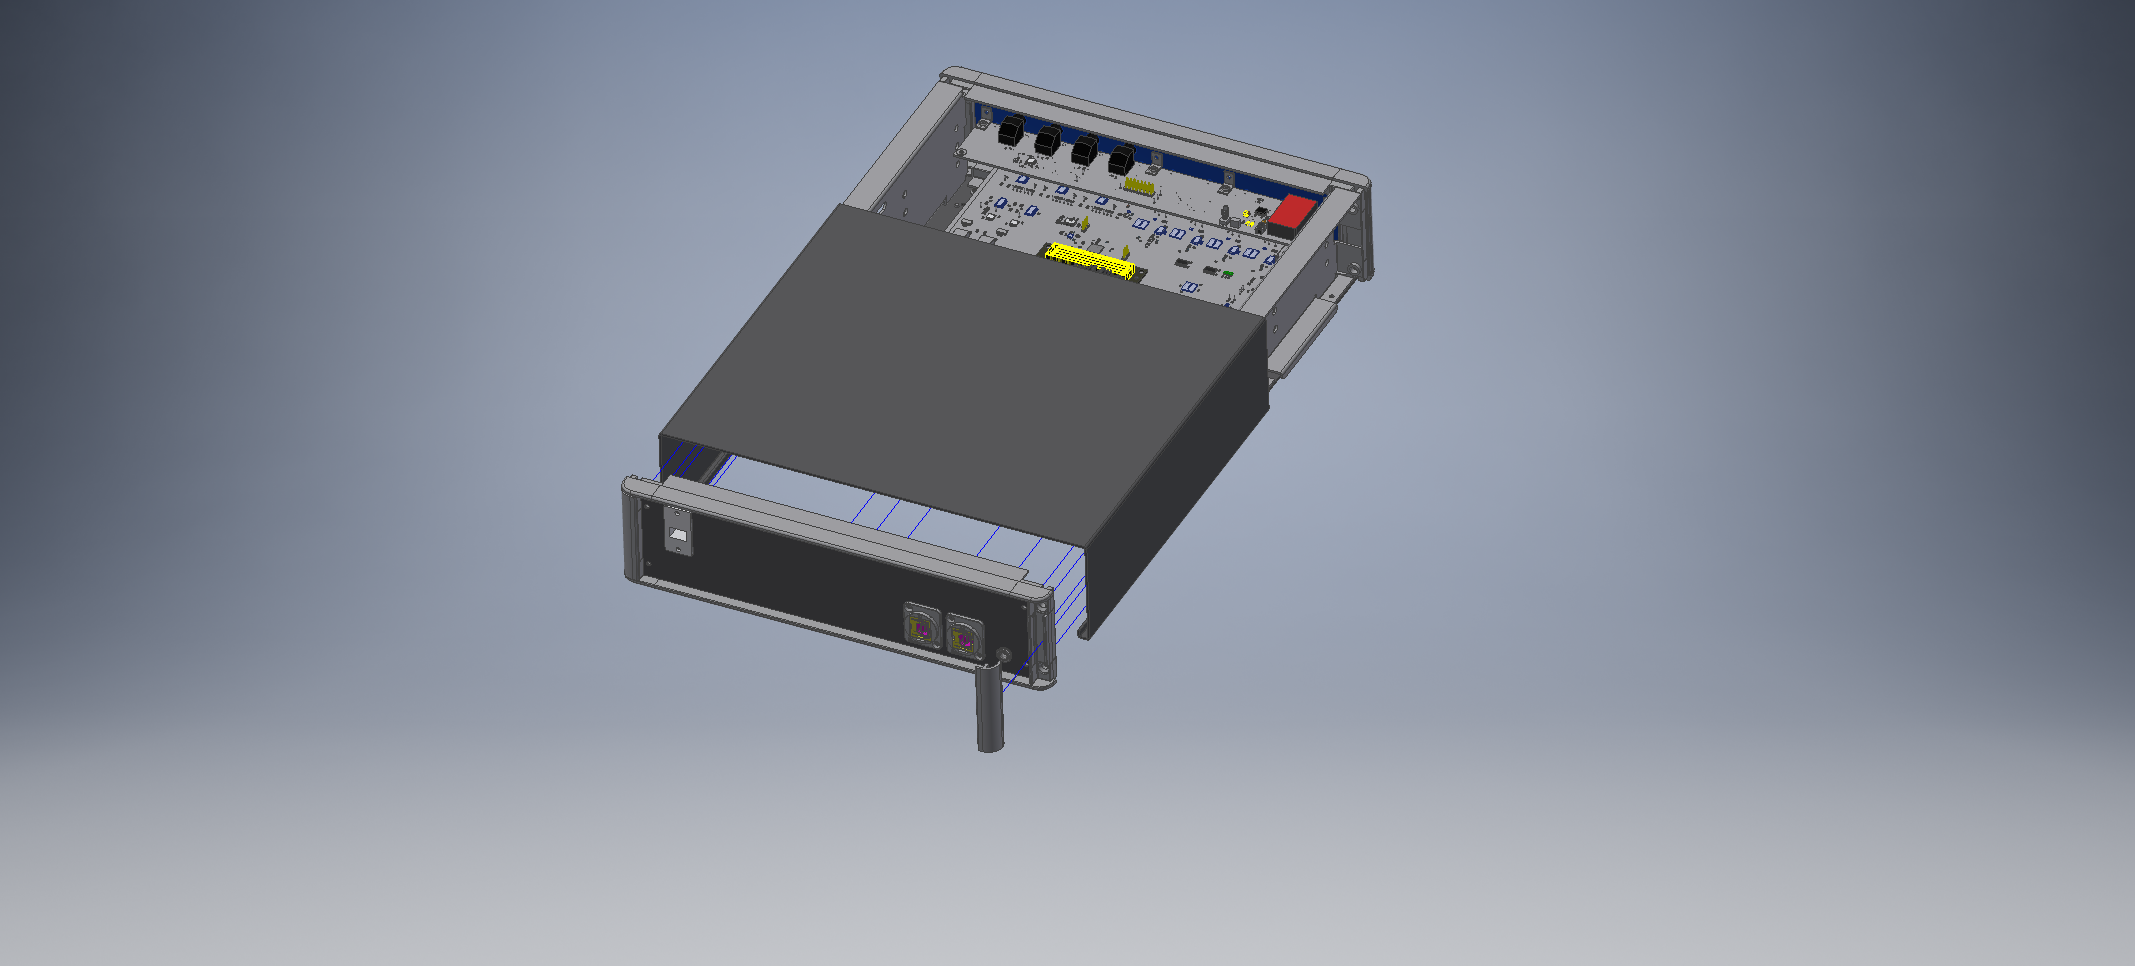
\includegraphics[width=.45\textwidth]{./Images/View5.png}}
    \caption{Steps to remove the cover from the unit.}
    \label{fig:dismantle}
\end{figure}
%\section{Preparation}
%Before powering the \gls{tlu} it is necessary to follow a few steps to ensure the board and the \gls{fpga} work correctly.\\
%
%Currently, it is recommended to use the following:
%\begin{itemize}
% \item MA-PM3-W-R5: Mars PM3 base board
% \item MA-AX3-35-1I-D8-R3: Marx AX3 module (hosts a Xilinx XC7A35T-1CSG324I )
% \item MA-PM3-ACC-BASE: Accessory kit, including a \gls{jtag} breakout board to connect Xilinx programming cables. Also includes a 12~V power supply to power the PM3.
%\end{itemize}
%
%\section{I/O voltage setting}
%The I/O pins of the PM3 can be configured to operate at 2.5~V or 3.3~V; the factory default is 2.5~V but the \brd requires 3.3~V logic. The user should make sure to select the appropriate voltage by operating on DIP-switch CFG-A/S1200 (pin 1 set to ON).\\For reference, a top view of the board is provided in the appendix at page~\pageref{ch:appendix}.\\
%\begin{alertinfo}{Warning}
%    Please double check the PM3 board manual for the correct way to change the I/O voltage setting. Enclustra has been changing their hardware recently.
%\end{alertinfo}
%
%\section{Xilinx programming cable}
%The \gls{jtag} pins on the PM3 are located on the header J800 (20-way, 2.54~mm pitch). The breakout board provided by Enclustra sits on top of the header and connects the pins to a 14-way Molex milli-grid header so that it is possible to plug the Xiling programming cable directly onto it. However, when the \brd is mounted on a base plate as shown in figure~\ref{fig:TLUplate}, the breakout board has to be detached from the PM3 because it interferes with the mounting screws.\\
%The connection between J800 and the breakout can be achieved by using two standard 20-way \gls{idc} cables as shown in figure~\ref{fig:XilinxCable}.
%\begin{figure}[h]
%  \centering
%  \includegraphics[width=.50\textwidth]{./Images/TLU_plate.jpg}
%  \caption{\brd and PM3 mounted on a base plate: in this configuration it is not possible to install the breakout board on the PM3 because the mountings screws are in the way.}\label{fig:TLUplate}
%\end{figure}
%\begin{figure}
%  \centering
%  \includegraphics[width=.80\textwidth]{./Images/XilinxCable.jpg}
%  \caption{Connecting the Xilinx programming cable to the PM3 in an ugly (but effective) way.}\label{fig:XilinxCable}
%\end{figure}

\chapter{TLU Hardware}\label{ch:hardware}
Board \brd is an evolution of the miniTLU designed at the \gls{uob}. The board shares a few features with the miniTLU but also introduces several improvements. This chapter illustrates the main features of the board to provide a general view of its capabilities and an understanding of how to operate it in order to communicate with the \gls{dut}s.

\section{Inputs and interfaces}\label{ch:hwDUT}
\subsubsection{FMC}
The board must be plugged onto a \gls{fmc} carrier board with an \gls{fpga} in order to function correctly. The connection is achieved using a low pin count \gls{fmc} connector. The list of the pins used and the corresponding signal within the \gls{fpga} are provided in appendix at page~\pageref{ch:appendix}.\\

\subsubsection{Device under test}\label{ch:dut}
The \gls{dut}s are connected to the \gls{tlu} using standard size \gls{hdmi} connectors\footnote{In the miniTLU hardware these were mini \gls{hdmi} connectors.}.\\
In the current version of the hardware, up to four \gls{dut}s can be connected to the board. In this document the connectors will be referred to as \verb|HDMI1|, \verb|HDMI2|, \verb|HDMI3| and \verb|HDMI4|.\\
The connectors operate with 3.3~V \gls{lvds} signals and are bi-directional, i.e. any differential pair can be configured to be an output (signal from the TLU to the DUT) or an input (signals from the DUT to the TLU) by using half-duplex line transceivers. Figure~\ref{fig:LVDSTransceiver} illustrates how the differential pairs are connected to the transceivers.
\begin{alertinfo}{Note}
    The input part of the transceiver is configured to be always on. This means that signals going \emph{into} the \gls{tlu} are always routed to the logic (\gls{fpga}). By contrast, the output transceivers have to be enabled and are off by default: signal sent from the logic to the \gls{dut}s cannot reach the devices unless the corresponding enable signal is active.
\end{alertinfo}
Table~\ref{tab:HDMIpins} shows the pin naming and the corresponding output enable signal. The clock pairs have two different enable signals to select the clock source (see section~\ref{ch:clock} for more details). In general only one of the clock sources should be active at any time.\\
The enable signals can be configured by programming two \gls{gpio} bus expanders via \gls{i2c} interface as described in section~\ref{ch:i2c}.
 \begin{table}[]
    \centering
    \caption{HDMI pin connections.}
    \label{tab:HDMIpins}
    \begin{tabular}{|l|l|l|}
    \hline
    \textbf{HDMI PIN} & \textbf{HDMI Signal Name} & \textbf{Enable Signal Name} \\ \hline
     &  &  \\ \hline
    1   & \verb|HDMI_CLK| & \begin{tabular}[c]{@{}l@{}}\verb|ENABLE_CLK_TO_DUT|\\ or\\ \verb|ENABLE_DUT_CLK_FROM_FPGA|\end{tabular} \\ \hline
    2   & \verb|GND|       & -- \\ \hline
    3   & \verb|HDMI_CLK| * & \begin{tabular}[c]{@{}l@{}}\verb|ENABLE_CLK_TO_DUT|\\ or\\ \verb|ENABLE_DUT_CLK_FROM_FPGA|\end{tabular} \\ \hline
    4   & \verb|CONT|      & \verb|ENABLE_CONT_FROM_FPGA| \\ \hline
    5   & \verb|GND|       & -- \\ \hline
    6   & \verb|CONT*|     & \verb|ENABLE_CONT_FROM_FPGA| \\ \hline
    7   & \verb|BUSY|      & \verb|ENABLE_BUSY_FROM_FPGA| \\ \hline
    8   & \verb|GND|       & -- \\ \hline
    9   & \verb|BUSY*|     & \verb|ENABLE_BUSY_FROM_FPGA| \\ \hline
    10  & \verb|SPARE|     & \verb|ENABLE_SPARE_FROM_FPGA| \\ \hline
    11  & \verb|GND|       & -- \\ \hline
    12  & \verb|SPARE*|    & \verb|ENABLE_SPARE_FROM_FPGA| \\ \hline
    13  & n.c.      &  \\ \hline
    14  & \verb|HDMI_POWER| & -- \\ \hline
    15  & \verb|TRIG|      & \verb|ENABLE_TRIG_FROM_FPGA| \\ \hline
    16  & \verb|TRIG*|     & \verb|ENABLE_TRIG_FROM_FPGA| \\ \hline
    17  & \verb|GND|       &  \\ \hline
    18  & n.c.      &  \\ \hline
    19  & n.c.      &  \\ \hline
    \end{tabular}
\end{table}
\begin{figure}
  \centering
  \includegraphics[width=.80\textwidth]{./Images/LVDS_transceiver.pdf}
  \caption{Internal configuration of the HDMI pins for the DUTs. The path from the DUT to the FPGA is always active. The path from the FPGA to the DUT can be enabled or disabled by the user.}\label{fig:LVDSTransceiver}
\end{figure}\\
In terms for functionalities, the four \gls{hdmi} connectors are identical with one exception: the clock signal from \verb|HDMI4| can be used as reference for the clock generator chip mounted on the hardware. For more details on this functionality refer to section~\ref{ch:clock}.

\subsubsection{SFP cage}
\brd hosts a \gls{sfp} cafe and a \gls{cdr} chip that can be used to decode a data stream over optical/copper interface. The data from the stream is routed to the \gls{fpga} while the clock can be fed to the Si5345 to provide a clock reference.

\section{Clock LEMO}
The board hosts a two-pin LEMO connector that can be used to provide a reference clock to the clock generator (see section~\ref{ch:clock}) or to output the clock from the \gls{tlu} to the external world, for instance to use it as a reference for another \gls{tlu}. The signal level is 3.3~V \gls{lvds}.\\
As for the differential pairs of the \gls{dut}s, the pins of this connector are wired to a transceiver configured to always accept the incoming signals. The outgoing direction must be enabled by using the \verb|ENABLE_CLK_TO_LEMO| signal, which can be configured using the bus expander described in in section~\ref{ch:i2c}.

\section{Trigger inputs}
Board \brd can accept up to six trigger inputs over the LEMO connectors labelled \verb|IN_1|, \verb|IN_2|, \verb|IN_3|, \verb|IN_4|, \verb|IN_5| and \verb|IN_6|. The \brd uses internal high-speed\footnote{500$\pm$30~ps propagation delay.} discriminators to detect a valid trigger signal. The voltage thresholds can be adjusted independently for each input in a range from -1.3~V to +1.3~V with 40~$\mu$V resolution.\\
The adjustment is performed by writing to two 16-bit \gls{dac}s via \gls{i2c} interface as described in section~\ref{ch:i2c}.\\
The \gls{dac}s can either use an internal reference voltage of 2.5~V or an external one of 1.3~V provided by the \gls{tlu}: it is recommended to choose the external one by configuring the appropriate register in the devices.\\
The correspondence between DAC slave and thresholds is shown in table~\ref{tab:DACOutputs}.
\begin{table}[]
\centering
\caption{DAC outputs and corresponding threshold inputs.}
\label{tab:DACOutputs}
\begin{tabular}{|l|c|c|}
\hline
                     & \multicolumn{2}{c|}{Output}                                                        \\ \hline
                     & \multicolumn{1}{l|}{\textbf{DAC2(Ic2)}} & \multicolumn{1}{l|}{\textbf{DAC1 (Ic1)}} \\ \hline
\textbf{Threshold 0} & 1                                       &                                          \\ \hline
\textbf{Threshold 1} & 0                                       &                                          \\ \hline
\textbf{Threshold 2} &                                         & 3                                        \\ \hline
\textbf{Threshold 3} &                                         & 2                                        \\ \hline
\textbf{Threshold 4} &                                         & 1                                        \\ \hline
\textbf{Threshold 5} &                                         & 0                                        \\ \hline
\end{tabular}
\end{table}


\section{I$^{2}$C slaves}\label{ch:i2c}
The \gls{i2c} interface on the \brd can be used to configured several features of the board.\\
Table~\ref{tab:I2C addresses} lists all the valid addresses and the corresponding slave on the board. The Enclustra lines refer to slaves located on the PM3 board; these slaves can be ignored with the exception of the bus expander. The Enclustra expander is used to enable/disable the \gls{i2c} lines going to the \gls{fmc} connector.
\begin{alertinfo}{Note}
    After a power cycle the Enclustra expander is configured to disable the \gls{i2c} interface pins. This means that it is impossible to communicate to any \gls{i2c} slave on the \gls{tlu} until the expander has been enabled.\\
    The interface is enable by setting bit 7 to 0 on register 0x01 of the Enclustra expander.
\end{alertinfo}
\begin{table}[]
    \centering
    \caption{I$^{2}$C addresses of the TLU. }
    \label{tab:I2C addresses}
    \begin{tabular}{|l|l|l|l|}
    \hline
    \textbf{CHIP} & \textbf{ID} & \textbf{FUNCTION}        & \textbf{ADDRESS} \\ \hline
    IC1           & AD5665RBRUZ & DAC1                     & 0x1F             \\ \hline
    IC2           & AD5665RBRUZ & DAC2                     & 0x13             \\ \hline
    IC5           & 24AA025E48T & EEPROM                   & 0x50             \\ \hline
    IC6           & PCA9539PW   & I2C Expander1            & 0x74             \\ \hline
    IC7           & PCA9539PW   & I2C Expander2            & 0x75             \\ \hline
    IC8           & ADN2814ACPZ & CDR                      & 0x60             \\ \hline
    IC8\_9        & Si5345A     & Clock Generator          & 0x68             \\ \hline
    \multicolumn{4}{|l|}{Enclustra slaves}                                                    \\ \hline
                  &             & Enclustra Bus Expander   & 0x21             \\ \hline
                  &             & Enclustra System Monitor & 0x21             \\ \hline
                  &             & Enclustra EEPROM         & 0x54             \\ \hline
                  &             & Enclustra slave          & 0x64             \\ \hline
\end{tabular}
\end{table}
Once the interface is enabled it is possible to read and write to the devices listed in the top part of table~\ref{tab:I2C addresses}.\\
The user should reference the manual of each individual component to determine the register that must be addressed. The rest of this section is meant to provide an overview of the slave functionalities.

\subsubsection{DAC}
Each \gls{dac} has four outputs that can be configured independently. \verb|DAC1| is used to configure the thresholds of the first four trigger inputs; \verb|DAC2| configures the remaining two thresholds.\\
The \gls{dac}s should be configured to use the \gls{tlu} voltage reference of 1.3~V. In these conditions, writing a value of 0x00000 to a \gls{dac} output will set the corresponding threshold to -1.3~V while a value of 0xFFFF will set it to +1.3~V.

\subsubsection{EEPROM}
The \gls{eeprom} located on the board contains a factory-set unique number, used to identify each \brd unequivocally. The number is comprised of six bytes written in as many memory locations.\\
The identifier is always in the form: \verb|0xD8 80 39 XX XX XX| with the top three bytes indicating the manufacturer and the bottom three unique to each device.

\subsubsection{Bus expander}
The expanders are used as electronic switched to enable and disable individual lines. Each expander has two 8-bit banks; the values of the bits, as well as their direction (input/output) can be configured via the \gls{i2c} interface. For the purpose of the \gls{tlu}, all the expander pins should be configured as outputs since they must drive the enable signals on the \gls{dut} transceivers.

\subsubsection{Clock and data recovery chip}
The \gls{cdr} is used in conjunction with the \gls{sfp} cage to recover data and clock from the incoming bit stream. The functionality has not yet been implemented in the firmware so the \gls{i2c} slave can be ignored for now.

\subsubsection{Clock generator}
The clock for \brd can be generated using various external or internal references (see section~\ref{ch:clock} for further details). In order to reduce any jitter from the clock source and to provide a stable clock, the board hosts a Si5345 clock generator that needs to be configured via \gls{i2c} interface.\\
The configuration involves writing $\thicksim$380 register values. A configuration file, containing all the register addresses and the corresponding values, can be generated using the ClockBuilder tool available from \href{http://www.enclustra.com/en/home/}{Silicon Labs}.\\
The registers addresses between 0x026B and 0x0272 contain user-defined values that can be used to identify the configuration version: it is advisable to check those registers and check that they contain the correct code to ensure that the chip is configured according to the \gls{tlu} specifications. As an indication, files generated for the current version of the \gls{tlu} should have a configuration identifier in the form \verb|TLU1E_XX|, where \verb|XX| is a sequential number.\\
\begin{alertinfo}{\gls{tlu} Producer}
    When using the \gls{tlu} producer to configure hardware, the location of the configuration file can be specified by setting the \texttt{CLOCK\_CFG\_FILE} value in the \emph{conf} file for the producer.\\
    If no value is specified, the software will look for the configuration file \texttt{../conf/confClk.txt} i.e. if the \texttt{euRun} binary file is located in \texttt{./eudaq/bin}, then the default configuration file should reside in \texttt{./eudaq/conf}. The configuration will produce an error if the file is not found.
\end{alertinfo}

\section{Power module and led}\label{ch:frontpanel}
The \gls{led}s and \gls{pmt} connectors on the front panel are part of an auxiliary board installed together with the \brd. All the functionalities on the board, such as the indicators and the \gls{dac} are controlled via \gls{i2c} bus.\\
Is the \gls{tlu} is controlled using EUDAQ, the \gls{dac} can be steered by means of a parameter in the configuration file (see section~\ref{ch:EUDAQPar} for details).\\
Three green \gls{led} on the front panel are used to indicate the presence of power (+12 V) and the correct functioning of the +5 V and -5 V voltage regulators. Further indicators are assigned to the \gls{hdmi} and trigger inputs to provide information on their status. These indicators are \gls{rgb}. At the moment there is not defined scheme to assign a meaning to each colour.\\
The LEMO connectors used to power the \gls{pmt}s are wired according to the following scheme, inherited from what already in use in beam telescopes (FIX THIS):
\begin{enumerate}
  \item POWER: +12~V
  \item not connected
  \item CONTROL, voltage signal from 0 to +1~V
  \item GND
\end{enumerate}
\begin{alertinfo}{\gls{tlu} Control voltage on modified units}
   Some users requested the possibility to use different types of \gls{pmt}s. To enable this, a few power modules have been modified to provide +5~V (instead of +12~V) and to have a maximum control voltage of 1.1~V (instead of 1~V).\\
   The modified units are clearly labelled and use different style of \gls{pmt} connectors, so that confusion should be minimized. 
\end{alertinfo}
\chapter{Clock}\label{ch:clock}
The \gls{tlu} can use various sources to produce a stable 40~MHz clock\footnote{For some applications a 50~MHz clock will be required instead}. A \gls{lvpecl} crystal provides the reference 50~MHz clock for a Si5345A jitter attenuator. The Si5345A can accept up to four clock sources and use them to generate the required output clocks.\\
In \brd the possible sources are: differential LEMO connector LM1\_9, one of the four \gls{hdmi} connectors (\verb|HDMI4|), a \gls{cdr} chip connected to the \gls{sfp} cage. The fourht input is used to provide a zero-delay feedback loop.\\
The low-jitter clock generated by the Si5345A can be distributed to up to ten recipients. In the \gls{tlu} these are: the four \gls{dut}s via \gls{hdmi} connectors, the differential LEMO cable, the \gls{fpga},  connector J1 as a differential pair (pins 4 and 6) and as a single ended signal (pin 8). The final output is connected to the zero-delay feedback loop. Note that it is possible to program the clock chip to generate a different frequency for each of its outputs.\\
The \gls{dut}s can receive the clock either from the Si5435A or directly from the \gls{fpga}: when provided by the clock generator, the signal name is \verb|CLK\_TO\_DUT| and is enabled by signal \verb|ENABLE_CLK_TO_DUT|; when the signal is provided directly from the \gls{fpga} the line used is \verb|DUT_CLK_FROM_FPGA| and is enabled by \verb|ENABLE_DUT_CLK_FROM_FPGA|.\\
The firmware uses the clock generated by the Si5345A except for the block \verb|enclustra_ax3_pm3_infra| which relies on a crystal mounted on the Enclustra board to provide the IPBus functionalities (in this way, at power up the board can communicate via IPBus even if the Si5345A is not configured).

\section{Input selection}
The Si5345 has four inputs that can be selected to provide the clock alignment; the selection can be automatic or user-defined. For further details on this aspect the user should consult the \href{https://www.silabs.com/documents/public/data-sheets/Si5345-44-42-D-DataSheet.pdf}{chip documentation}\footnote{https://www.silabs.com/documents/public/data-sheets/Si5345-44-42-D-DataSheet.pdf}.

\begin{table}[]
\small
\centering
\caption{Si5345  Input Selection Configuration.}
\label{tab:si5345inputs}
\begin{tabular}{|l|l|l|}
\hline
\textbf{Register Name} & \textbf{Hex Address {[}Bit Field{]}} & \textbf{Function}                                                                                                                                                                                                                              \\ \hline
CLK\_SWITCH\_MODE      & 0x0536{[}1:0{]}                      & \begin{tabular}[c]{@{}l@{}}Selects manual or automatic switching modes.\\ Automatic mode can be revertive or non-revertive.\\ Selections are the following:\\00 Manual\\01 Automatic non-revertive\\02 Automatic revertive\\03 Reserved\end{tabular} \\ \hline
IN\_SEL\_REGCTRL       & 0x052A {[}0{]}                       & \begin{tabular}[c]{@{}l@{}}0 for pin controlled clock selection\\ 1 for register controlled clock selection\end{tabular}                                                                                                                       \\ \hline
IN\_SEL                & 0x052A {[}2:1{]}                     & \begin{tabular}[c]{@{}l@{}}0 for IN0\\ 1 for IN1\\ 2 for IN2\\ 3 for IN3 (or FB\_IN)\end{tabular}                                                                                                                                              \\ \hline
\end{tabular}
\end{table}


\section{Logic clocks registers}\label{ch:logicClock}
LogicClocksCSR: in the new TLU the selection of the clock source is done by programming the Si5345. As a consequence, there is no reason to write to this register. Reading it back returns the status of the PLL on bit 0, so this should read 0x1. 
\chapter{DUT signals}\label{ch:DUTsignals}
In the old versions of the \gls{tlu} the direction of the signals on the \verb|HDMI*| connectors were pre-defined. The new hardware has separate lines for signals going into the \gls{tlu} and signals out of the \gls{tlu}. See section~\ref{ch:hwDUT} for further details. \\ 
\include{ch_TLU_triggerInputs}
\include{ch_EventBuffer}
\chapter{Functions}\label{ch:functions}
The following is a list of files containing the code for the \gls{tlu}:
\begin{itemize}
  \item \verb|./eudaq2/user/eudet/misc/aida_tlu_test.ini|:\newline initialization file for the hardware. The location of the file can be passed to the EUDAQ code in the \gls{gui}.
  \item \verb|./eudaq2/user/eudet/misc/aida_tlu_test.conf|:\newline configuration file. It contains all the parameters to be loaded in the \gls{tlu} at the beginning of the run. If this file is not found, EUDAQ will use a list of default settings. The location of the file (and its name) can be passed to the EUDAQ code in the \gls{gui}.
  \item \verb|./eudaq2/user/eudet/misc/aida_tlu_test_connection.xml|:\newline define the IP address and address map of the \gls{tlu}. The one listed is the default location for the file. A different location can be specified with the \verb|ConnectionFile| option in the \emph{conf} file for the \gls{tlu}.
  \item \verb|./eudaq2/user/eudet/misc/aida_tlu_test_address.xml|:\newline address map for the \gls{tlu}. The location of the file is specified in the \verb|fmctlu_connection.xml| file.
  \item \verb|./eudaq2/user/eudet/misc/aida_tlu_test_clock_config.txt|:\newline configuration for the Si5345 clock chip. In order for the hardware to work a configuration file must be present. Those listed are the default name and location for the file; a different file can be specified with the \verb|CLOCK_CFG_FILE| option in the \emph{conf} file for the \gls{tlu}.
  \item \verb|./eudaq2/user/eudet/module/src/FMCTLU_Producer.cc|:\newline eudaq producer for the \gls{tlu}. Contains the methods to initialize, configure, start, stop the \gls{tlu} producer.
  \item \verb|./eudaq2/user/eudet/hardware/src/AidaTluController.cc|:\newline Contains the definition of the hardware class for the \gls{tlu} and the methods to set and read from its hardware, such as clock chip, DAC, etc. This lever is abstract with respect to the actual hardware, so that if a future version of the board uses different components it should be possible to re-use this code.
  \item \verb|./eudaq2/user/eudet/hardware/include/AidaTluController.hh|:\newline Headers for the controller.
  \item \verb|./eudaq2/user/eudet/hardware/src/AidaTluController.cxx|:\newline Executable for the controller.
  \item \verb|./eudaq2/user/eudet/hardware/src/AidaTluHardware.cc|:\newline This is the code that deals with the actual hardware on the \gls{tlu}, and contains specific instructions for the chips mounted in the current version. It contains several classes for the ADC, the clock chip, the I/O expanders etc.
  \item \verb|./eudaq2/user/eudet/hardware/include/AidaTluHardware.hh|:\newline Header for the hardware.
  \item \verb|./eudaq2/user/eudet/hardware/src/AidaTluI2c.cc|:\newline core functions used to read and write from \gls{i2c} compatible slaves.
  \item \verb|./eudaq2/user/eudet/hardware/include/AidaTluI2c.hh|:\newline Headers for the \gls{i2c} core.
\end{itemize}

\section{Functions}
\begin{description}
  \item[enableClkLEMO] Enable or disable the output clock to the differential LEMO connector.
  \item[enableHDMI] Set the status of the transceivers for a specific HDMI connector. When enable= False the transceivers are disabled and the connector cannot send signals from FPGA to the outside world. When enable= True then signals from the FPGA will be sent out to the HDMI.\\ In the configuration file use \verb|HDMIx_on = 0| to disable a channel and \verb|HDMI1_on = 1| to enable it (x can be 1, 2, 3, 4).\\
      NOTE: the other direction is always enabled, i.e. signals from the DUTs are always sent to the FPGA.\\
      NOTE: Clock source must be defined separately using SetDutClkSrc (DUTClkSrc in python script).\\
      NOTE: this is called \verb|DUTOutputs| on the python scripts.
  \item[GetFW] dsds
  \item[getSN] dsd
  \item[I2C\_enable] dsd
  \item[InitializeClkChip]
  \item[InitializeDAC]
  \item[InitializeIOexp]
  \item[InitializeI2C]
  \item[PopFrontEvent]
  \item[ReadRRegister]
  \item[ReceiveEvents]
  \item[ResetEventsBuffer]
  \item[SetDutClkSrc] Set the clock source for a specific \gls{hdmi} connector. The source can be set to 0 (no clock), 1 (Si5345) or 2 (FPGA). In the configuration file use \verb|HDMIx_on = N| to select the source (x can be 1, 2, 3, 4, N is the clock source).\\
      NOTE: this is called \verb|DUTClkSrc| on python scripts.
  \item[SetPulseStretchPk] Takes a vector of six numbers, packs them (5-bits each) and sends them to the PulseStretch register.
  \item[SetThresholdValue]
  \item[setTrgPattern] Writes two 32-bit words to define the trigger pattern for the inputs. See section~\ref{ch:triggerinputs} for details.
  \item[SetWRegister]
  \item[SetUhalLogLevel]
\end{description}



\include{ch_TLU_IPBusRegs}
\chapter{EUDAQ Parameters}\label{ch:EUDAQPar}
List of parameters that are parsed by the EUDAQ run control \gls{gui} to configure the \gls{tlu}.\\
The parameters must be included in the INI or CONF file passed to the main window (see~fig.\ref{fig:EUDAQGui}).
\begin{figure}
  \centering
  \includegraphics[width=.90\textwidth]{./Images/RunControlGUI.jpg}
  \caption{Main user iterface of the EUDAQ framework.}
  \label{fig:EUDAQGui}
\end{figure}\\
Not all parameters are needed; if one of the parameters is not present in the files, the code will generally assume a default value, indicated in brackets in the following document \verb|[type, default]|.
\begin{alertinfo}{Case sensitiveness}
    All parameters names are case sensitive!\\
    Please ensure to use the correct capitalization.\\
    A misspelled parameter will be ignored and its default value will be used instead.
\end{alertinfo}

\section{INI file}
\begin{description}
  \item[initid] \verb|[string, "0"]| Does not serve any purpose in the code but can be useful to identify configuration settings used in a specific run. As an example, the user can write a mnemonic such as `Testbeam\_April' or `2017\_10\_init' to help identifying a specific configuration. EUDAQ will store this information in the run data.
  \item[ConnectionFile] \verb|[string, "file://./FMCTLU_connections.xml"]| Name of the xml file used to store the information required to communicate with the hardware, such as its IP address and the location of the address map. The default location indicates a file that must be located in the \texttt{bin} folder.
  \item[skipini] \verb|[int, 0]| When this flas is set, the producer will skip the whole initialization phase for the \gls{tlu}. This can be useful to avoid disturbing any other piece of hardware connected to the unit, as it avoid re-initializing the \gls{dac}s, \gls{hdmi} connectors, clock chip, etc.
  \item[DeviceName] \verb|[string, "fmctlu.udp"]| The name of the type of hardware to be contacted by the IPBus.
  \item[TLUmod] \verb|[string, "1e"]| Version of the \gls{tlu} hardware. Reserved for future use.
  \item[nDUTs] \verb|[positive int, 4]| Number of \gls{dut} in the current \gls{tlu}. This is for future upgrades and should not require editing by the user.
  \item[nTrgIn] \verb|[positive int, 6]| Number of trigger inputs in the current \gls{tlu}. This is for future upgrades and should not require editing by the user.
  \item[I2C\_COREEXP\_Addr] \verb|[positive int, 0x21]| \gls{i2c} address of the core expander mounted on the Enclustra board. This is not required if a different \gls{fpga} is used. See section~\ref{ch:i2c} for further details.
  \item[I2C\_CLK\_Addr] \verb|[positive int, 0x68]| \gls{i2c} address of Si5345 clock generator installed on the \gls{tlu}.
  \item[I2C\_DAC1\_Addr] \verb|[positive int, 0x13]| \gls{i2c} address of \gls{dac} installed on the \gls{tlu}. The \gls{dac} is used to configure the threshold of the trigger inputs.
  \item[I2C\_DAC2\_Addr] \verb|[positive int, 0x1F]| \gls{i2c} address of \gls{dac} installed on the \gls{tlu}. The \gls{dac} is used to configure the threshold of the trigger inputs.
  \item[I2C\_ID\_Addr] \verb|[positive int, 0x50]| \gls{i2c} address of the unique ID \gls{eeprom} installed on the \gls{tlu}. The chip is used to provide a unique identifier to each kit.
  \item[I2C\_EXP1\_Addr] \verb|[positive int, 0x74]| \gls{i2c} address of the bus expander used to select the direction of the \gls{hdmi} pins on the board.
  \item[I2C\_EXP2\_Addr] \verb|[positive int, 0x75]| \gls{i2c} address of the bus expander used to select the direction of the \gls{hdmi} pins on the board.
  \item[I2C\_DACModule\_Addr] \verb|[positive int, 0x1C]| \gls{i2c} address of the \gls{dac} installed on the power module and used to control the \gls{pmt} outputs.
  \item[PMT\_vCtrlMax] \verb|[float, 1]| value, in volts, of the maximum control voltage for the \gls{pmt}s. For EUDET telescopes this should normally be left to 1~V. If the \gls{tlu} is going to be used with different \gls{pmt}s, then a new value can be used but the hardware must be tweaked accordingly by changing the voltagi divider on the power module.
  \item[I2C\_EXP1Module\_Addr] \verb|[positive int, 0x76]| \gls{i2c} address of the first expander used to control the indicators on the power module.
  \item[I2C\_EXP2Module\_Addr] \verb|[positive int, 0x77]| \gls{i2c} address of the second expander used to control the indicators on the power module.
  \item[intRefOn] \verb|[boolean, false]| If true, the \gls{dac}s installed on the \gls{tlu} will use their internal voltage reference rather than the one provide externally.
  \item[VRefInt] \verb|[float, 2.5]| Value in volts for the internal reference voltage of the \gls{dac}s. The voltage is chosen by the chip manufacturer. This is only used if \verb|intRefOn= true|.
  \item[VRefExt] \verb|[float, 1.3]| Value in volts for the external reference voltage of the \gls{dac}s. The voltage is determined by a circuit on the \gls{tlu} and the value of this parameter must reflect such voltage. This is only used if \verb|intRefOn= false|.
  \item[CONFCLOCK] \verb|[boolean, true]| If true, the clock chip Si5345 will be re-configured when the INIT button is pressed (see figure~fig.\ref{fig:EUDAQGui}). The chip is configured via \gls{i2c} interface using a specific text file (see next parameter). After a power cycle, the chip is its default state and must be reconfigured to operate the \gls{tlu} correctly\footnote{As long as the unit is powered, the clock chip will maintain its setup, so the user can set this flag to 0 after the first initialization, in order to save time.}.
  \item[CLOCK\_CFG\_FILE] \verb|[string, "./../user/eudet/misc/fmctlu_clock_config.txt"]| Name of the text file used to store the configuration values of the Si5345. The file can be generate using the Clockbuilder Pro software provided by \href{https://www.silabs.com/products/development-tools/software/clock}{SiLabs}.
\end{description}

\section{CONF file}
\begin{description}
  \item[confid] \verb|[string, "0"]| Does not serve any purpose in the code but can be useful to identify configuration settings used in a specific run. EUDAQ will store this information in the run data.
  \item[verbose] \verb|[int, 0]| Defines the level of output messages from the \gls{tlu}. 0= only errors (minimum), 1= warning (default), 2= info, 3= all.
  \item[skipconf] \verb|[int, 0]| When this flag is set, EUDAQ will skip the whole configuration phase for the \gls{tlu}. When the user configures the hardware in EUDAQ, the board will remain in its current state and no configuration parameter will be written. This can be useful to avoid disturbing other pieces of electronics.
  \item[HDMI1\_set] \verb|[unsigned int, 0b0001]| Defines the source of the signal on the pins for the \verb|HDMI1| connector. A 1 indicates that each pin pair is an driven by the \gls{tlu}, a 0 that they are left floating (with respect to the \gls{tlu}). This can be used to define the signal direction on each pin pair. The order of the pairs is as follow:\\
  bit 0= CONT, bit 1= SPARE, bit 2= TRIG, bit 3= BUSY.\\
  Note that the direction of the DUTClk pair is defined in a separate parameter (see HDMI\_clk).\\
  Example to configure the connector to work with an EUDET device:\\
  - in this configuration the BUSY line is driven by the device under test, so it is an input for the \gls{tlu} and should not be driven by it (bit 3= 0)\\
  - TRIGGER line is an output for the \gls{tlu} so is driven by it (bit 2= 1)\\
  - SPARE line is used to provide control signals, such as the reset signal to initialize the devices at the start of a run (\texttt{T$_0$}). It should be configured as driven by the \gls{tlu} (bit 1= 1)\\
  - CONT is used by the \gls{tlu} to issue control commands and should be configured as a signal driven by the \gls{tlu} (bit 0= 1).\\
  Therefore the value of this parameter would be 0x7 (b0111).
  \item[HDMI2\_set] \verb|[unsigned int, 0b0001]| Defines the direction of the pins for the \verb|HDMI2| connector.
  \item[HDMI3\_set] \verb|[unsigned int, 0b0001]| Defines the direction of the pins for the \verb|HDMI3| connector.
  \item[HDMI4\_set] \verb|[unsigned int, 0b0001]| Defines the direction of the pins for the \verb|HDMI4| connector.
  \item[HDMI1\_clk] \verb|[unsigned int, 1]| Defines if the DUTClk pair on the \gls{hdmi} connector must be driven by the \gls{tlu} and, if so, what clock source to use. A 0 indicates that the pins are not driven by the \gls{tlu}. 1 indicates that pins will by driven with the clock produced from the on-board clock chip Si5345. 2 indicates that the driving clock is obtained from the \gls{fpga}.\\
      Example to configure the connector to work with an EUDET device: in this scenario the clock is driven by the \gls{dut} so the parameter should be set to 0.
      Example to configure the connector to work with an AIDA device: in this scenario the clock is driven by the \gls{tlu} so the parameter should be set to either 1 or 2 (by default 1).
  \item[HDMI2\_clk] \verb|[unsigned int, 1]| Defines the driving signal on the corresponding \gls{hdmi} connector.
  \item[HDMI3\_clk] \verb|[unsigned int, 1]| Defines the driving signal on the corresponding \gls{hdmi} connector.
  \item[HDMI4\_clk] \verb|[unsigned int, 1]| Defines the driving signal on the corresponding \gls{hdmi} connector.
  \item[LEMOclk] \verb|[boolean, true]| Defines whether a driving clock is to be provided on the differential LEMO connector of the \gls{tlu}. By default (value= 1), the clock is driven from the clock chip. If the value is set to 0 no clock will be driven.
  \item[PMT1\_V] \verb|[float, 0.0]| Defines the control voltage for PMT 1, in volts. The value can range from 0 to 1 V.
  \item[PMT2\_V] \verb|[float, 0.0]| Defines the control voltage for PMT 2, in volts. The value can range from 0 to 1 V.
  \item[PMT3\_V] \verb|[float, 0.0]| Defines the control voltage for PMT 3, in volts. The value can range from 0 to 1 V.
  \item[PMT4\_V] \verb|[float, 0.0]| Defines the control voltage for PMT 4, in volts. The value can range from 0 to 1 V.
  \item[in0\_STR] \verb|[unsigned int, 0]| Defines the number of clock cycles used to stretch a pulse once a trigger is detected by the discriminator on input 0. This feature allows the user to modify the pulses that are then fed into the trigger logic within the \gls{tlu}.
      A minimum lenght of 6.25~ns is provided if the value is 0. Any extra clock cycle extend the pulse by 6.25~ns (160~MHz clock). An example of the effect on the stretch setting is shown in figure~\ref{Fig:exampleExtendedTriggers}.
  \item[in0\_DEL] \verb|[unsigned int, 0]| Defines the delay, in 160~MHz clock cycles, to be assigned to the discriminated pulse from input 0, in order to process the logic for the trigger. This can be used to compensate for differences in cable lengths for the signals used to create a trigger.
  \item[in1\_STR] \verb|[unsigned int, 0]| Same as \texttt{in1\_STR} but for input 1.
  \item[in1\_DEL] \verb|[unsigned int, 0]| Same as \texttt{in1\_DEL} but for input 1.
  \item[in2\_STR] \verb|[unsigned int, 0]| Same as \texttt{in1\_STR} but for input 2.
  \item[in2\_DEL] \verb|[unsigned int, 0]| Same as \texttt{in1\_DEL} but for input 1.
  \item[in3\_STR] \verb|[unsigned int, 0]| Same as \texttt{in1\_STR} but for input 3.
  \item[in3\_DEL] \verb|[unsigned int, 0]| Same as \texttt{in1\_DEL} but for input 1.
  \item[trigMaskHi] \verb|[unsigned int32, 0]| This word represents the most significative bits of the 64-bits used to determine the trigger mask.\\
        A detailed explanation of how to determine the correct word is provided in section~\ref{ch:triggerLogic}.
  \item[trigMaskLo] \verb|[unsigned int32, 0]| This word represents the least significative bits of the 64-bits used to determine the trigger mask.\\
        A detailed explanation of how to determine the correct word is provided in section~\ref{ch:triggerLogic}.
  \item[DUTMask]  \verb|[unsigned int, 0x1]| This mask indicates which \gls{hdmi} inputs have an AIDA device connected. Each of the lowest four bits correspond to a connector (bit 0= DUT1, bit 1= DUT2, bit 2= DUT3, bit 3= DUT4). If the bit is set to 1 the \gls{tlu} expects a device connected and exchanging signals according to the mode selected (see DUTMaskMode).
  \item[DUTMaskMode]  \verb|[unsigned int, 0xFF]| Defines the mode of operation of the device connected to a specific \gls{hdmi} port.\\
        Two bits are needed for each device, so bits 0,1 refer to \gls{hdmi}1, bits 2, 3 refer to \gls{hdmi}2, etc. Currently only the lower bit of each pair is needed to specify if the device is in AIDA mode (\texttt{bX1}) or EUDET mode (\texttt{bx0}).\\
        Example: to configure device 1 and 2 as EUDET and the rest as AIDA, the parameters should be set to 11-11-x0-x0, i.e. 0xF0 (but 0xFA, 0xF2 and 0xF8 would also work the same).\\
        See also section~\ref{ch:IPBus_DUT}.
  \item[DUTMaskModeModifier] \verb|[unsigned int, 0xF]| This mask only affects EUDET mode. Each of the lower 4 bits correspond to a device. If the device is in EUDET mode, it can assert DUTClk to produce a global veto in the triggers. This behaviour occurs if the corresponding bit is set to 1. If the bit is set to 0, asserting the DUTClk from the device will not produce a global veto.
  \item[DUTIgnoreBusy] \verb|[unsigned int, 0xF]| This mask tells the \gls{tlu} to ignore the BUSY signal from a specific device, either in AIDA or EUDET mode. If the device is in AIDA mode, this means that further triggers will be issued while the device is busy. If the device is in EUDET mode, this means that the \gls{tlu} will not pause while they are in the handshake phase. In turn, this means that the device will likely receive events where the trigger number does not increase sequentially by one.
  \item[DUTIgnoreShutterVeto] \verb|[unsigned int, 0x1]| Set bit to 1 to tell the \gls{dut} to ignore the shutter signal.
  \item[EnableRecordData] \verb|[boolean, true]| if set to 1, enable the data recording in the \gls{tlu}.
  \item[InternalTriggerFreq] \verb|[unsigned int, 0]| Defines the rate of the trigger generated internally by the \gls{tlu}, in Hz: if 0, the internal triggers are disabled. Any other value activates the internal trigger generator with frequency equal to the parameter. Values above 160~MHz are coerced to 160~MHz.
\end{description} 
\chapter{Control software}\label{ch:controlsw}
The preferred method to run the \gls{tlu} is by using the \href{https://github.com/eudaq/eudaq}{EUDAQ}\footnote{https://github.com/eudaq/eudaq} data acquisition framework.\\
A \gls{tlu} producer, based on C++, has been written to integrate the hardware in EUDAQ and is regularly pushed to the master repository. Checking out the latest EUDAQ software ensures to also have a stable version of the producer.\\
In addition to the EUDAQ producer, a set of Python scripts has been developed to enable users to configure and run the \gls{tlu} using a minimal environment without having to setup the whole data acquisition framework. The scripts are meant to reflect all the functionalities in the EUDAQ producers, i.e. using the scripts it should be possible to perform any operation available on the EUDAQ producer. However, they should only be used for local debugging and testing.\\
\begin{alertinfo}{Warning}
    When fixing bus or developing new software for the \gls{tlu}, priority will be given to ensure that the EUDAQ producer is patched first. As a consequence, there is a higher chance to find bugs in the Python scripts. 
\end{alertinfo}


\section{EUDAQ Producer}\label{ch:eudaqprod}
Current structure of a fmctlu producer event:
\lstset{language=XML}
\scriptsize
\begin{lstlisting}
<Event>
  <Type>2149999981</Type>
  <Extendword>171577627</Extendword>
  <Description>Ex0Tg</Description>
  <Flag>0x00000018</Flag>
  <RunN>0</RunN>
  <StreamN>0</StreamN>
  <EventN>0</EventN>
  <TriggerN>88</TriggerN>
  <Timestamp>0x0000000000000000  ->  0x0000000000000000</Timestamp>
  <Timestamp>0  ->  0</Timestamp>
  <Block_Size>0</Block_Size>
  <SubEvents>
    <Size>1</Size>
    <Event>
      <Type>2149999981</Type>
      <Extendword>3634980144</Extendword>
      <Description>TluRawDataEvent</Description>
      <Flag>0x00000010</Flag>
      <RunN>96</RunN>
      <StreamN>4008428646</StreamN>
      <EventN>88</EventN>
      <TriggerN>88</TriggerN>
      <Timestamp>0x0000000105b44f91  ->  0x0000000105b44faa</Timestamp>
      <Timestamp>4390670225  ->  4390670250</Timestamp>
      <Tags>
        <Tag>PARTICLES=89</Tag>
        <Tag>SCALER0=93</Tag>
        <Tag>SCALER1=93</Tag>
        <Tag>SCALER2=0</Tag>
        <Tag>SCALER3=0</Tag>
        <Tag>SCALER4=0</Tag>
        <Tag>SCALER5=0</Tag>
        <Tag>TEST=110011</Tag>
        <Tag>trigger=</Tag>
      </Tags>
      <Block_Size>0</Block_Size>
    </Event>
  </SubEvents>
</Event>
\end{lstlisting}
\normalsize
\begin{description}
  \item[Type] ??
  \item[ExtendWord] ??
  \item[Description]
  \item[Flag] Independent from producer. See the \href{https://github.com/eudaq/eudaq/blob/master/main/lib/core/include/eudaq/Event.hh#L87}{EUDAQ documentation} for details.
  \item[RunN]
  \item[StreamN]
  \item[EventN]
  \item[TriggerN] Both in the event and subevent this is written byt the producer with \verb|ev->SetTriggerN(trigger_n);|
  \item[Timestamp] The event timestamp is currently always 0. The subevent timestamps is written by the producer \verb|ev->SetTimestamp(ts_ns, ts_ns+25, false);|. The top line (0x0000000105b44f91, in the example) is coarse time stamp multiplied by 25, so it represents the time in nanoseconds. The bottom one (4390670225) is the same number but written in decimal format instead of hexadecimal.
  \item[PARTICLES] Number of pre-veto triggers recorded by the \gls{tlu}: the trigger logic can detect a valid trigger condition even when the unit is vetoed. In this case no trigger is issued to the \gls{dut}s but the number of such triggers is stored as number of particles. \verb|ev->SetTag("PARTICLES", std::to_string(pt));|
  \item[SCALER\#] Number of triggers edges seen by the specific discriminator. \verb|ev->SetTag("SCALER", std::to_string(sl));|
  \item[???] Event type from \gls{tlu} is missing?
  \item[???] Input trig, i.e. the actual firing inputs should be in TRIGGER but there seems to be nothing there
\end{description}

\section{Python scripts}
The scripts used to debug work locally with the \gls{tlu} are located in a dedicated folder in the \href{https://github.com/PaoloGB/firmware_AIDA/tree/master/TLU_v1e/scripts}{firmware repository}\footnote{https://github.com/PaoloGB/firmware\_AIDA/tree/master/TLU\_v1e/scripts} and rely on additional packages and software.
First of all, the user should download the \href{https://github.com/PaoloGB/firmware_AIDA/tree/master/packages}{packages} used to control the various components of the hardware\footnote{https://github.com/PaoloGB/firmware\_AIDA/tree/master/packages}. It is also necessary to have a local installation of \href{https://ipbus.web.cern.ch/ipbus/doc/user/html/index.html}{IPBUS and uHAL}\footnote{https://ipbus.web.cern.ch/ipbus/doc/user/html/index.html}.\\
Once all the necessary packages have been installed and the environment is set to point to the right folders, it is possible to run the \verb|startTLU_v1e.py| script to start an interface that allows to operate the \gls{tlu}.
 
\chapter{Appendix}\label{ch:appendix}
\section{Layout of Enclustra FPGA.}
\includepdf[link,pages={1}]{./Docs/PM3TopView.pdf}
\section{Connections between TLU and FPGA package.}
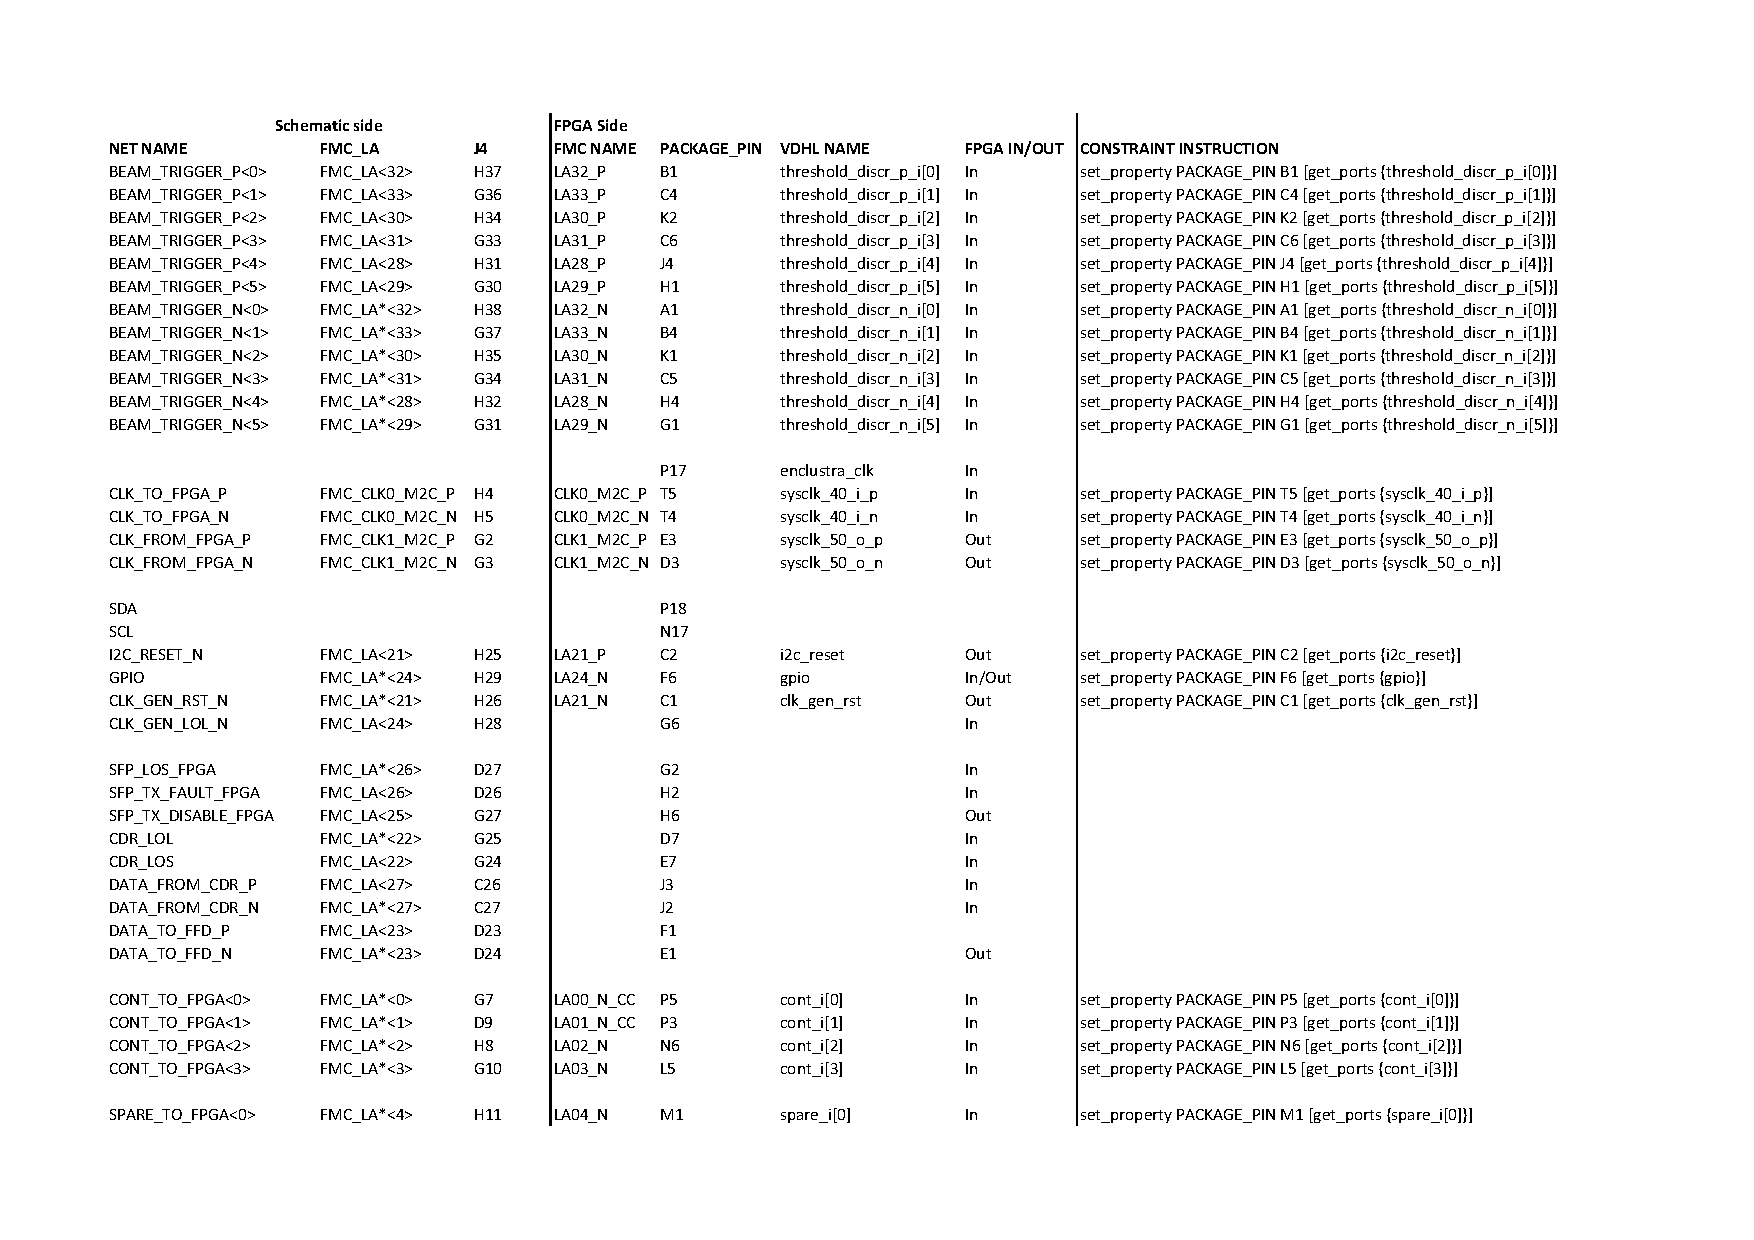
\includepdf[link,pages=-, angle=90]{./Docs/Connections.pdf}
\section{Schematics for main TLU electronics.}
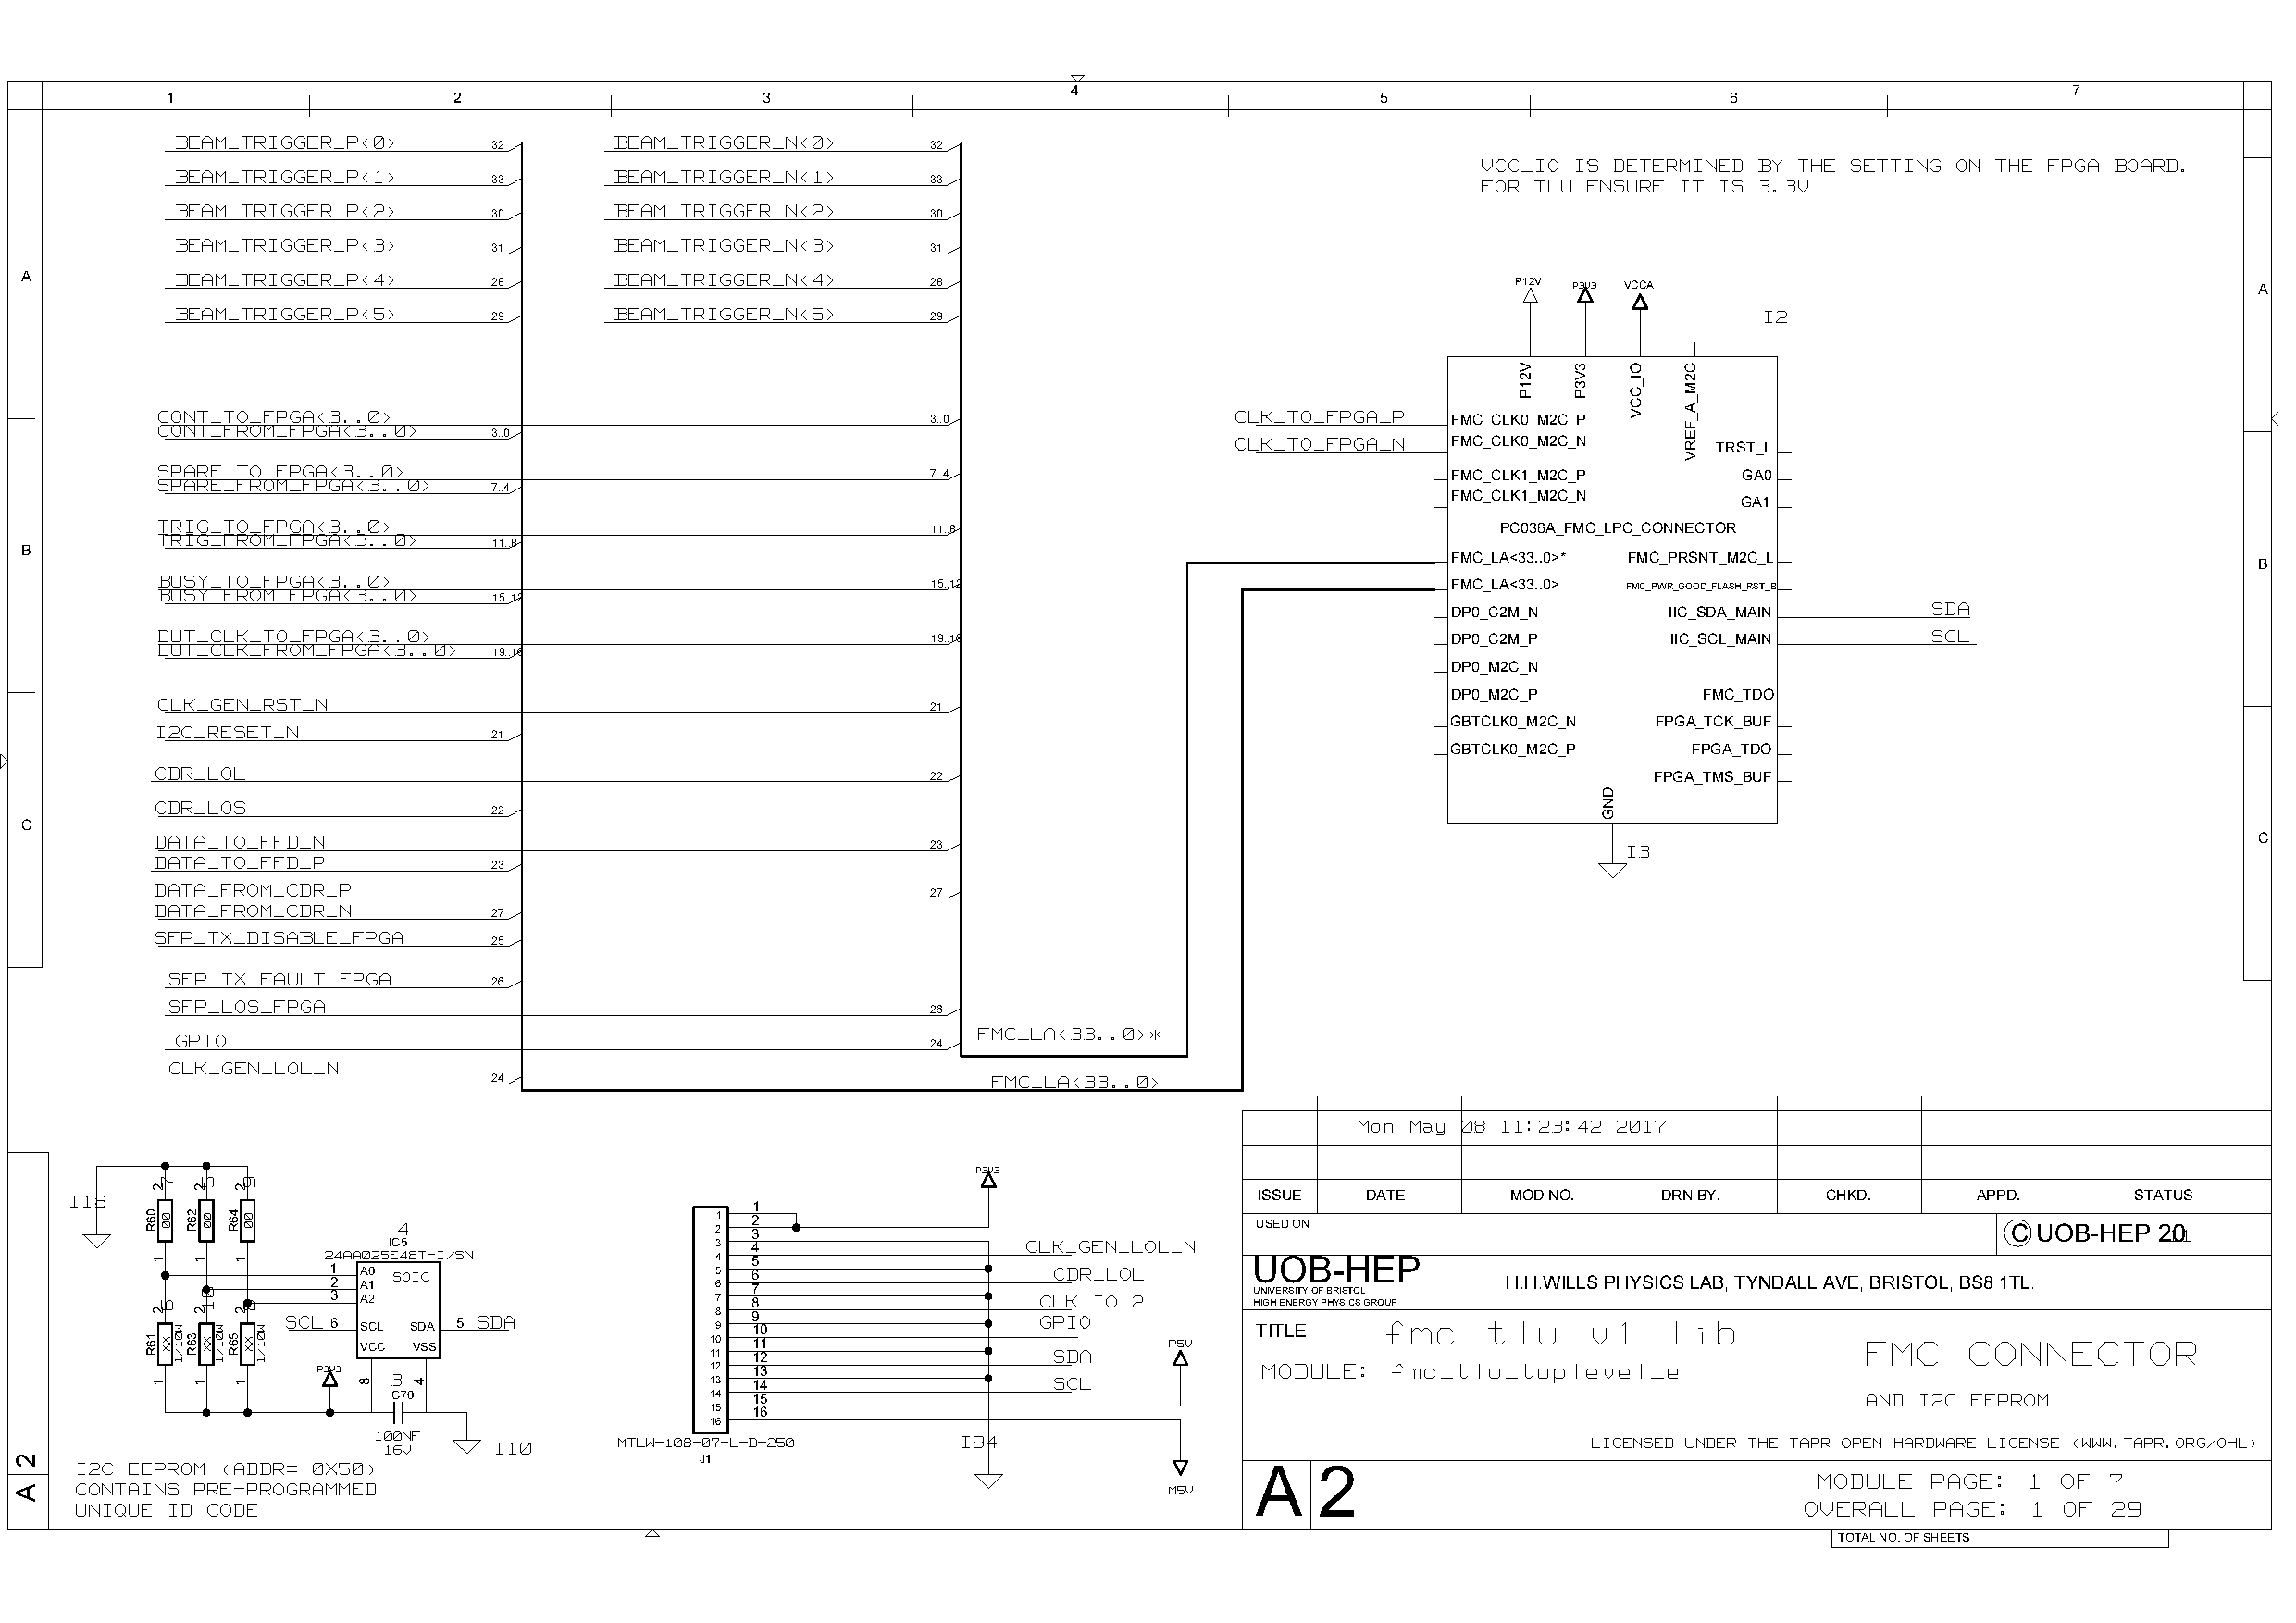
\includepdf[link,pages=-, angle=90]{./Docs/schematics.pdf} 
\section{Schematics for LED and PMT power module.}
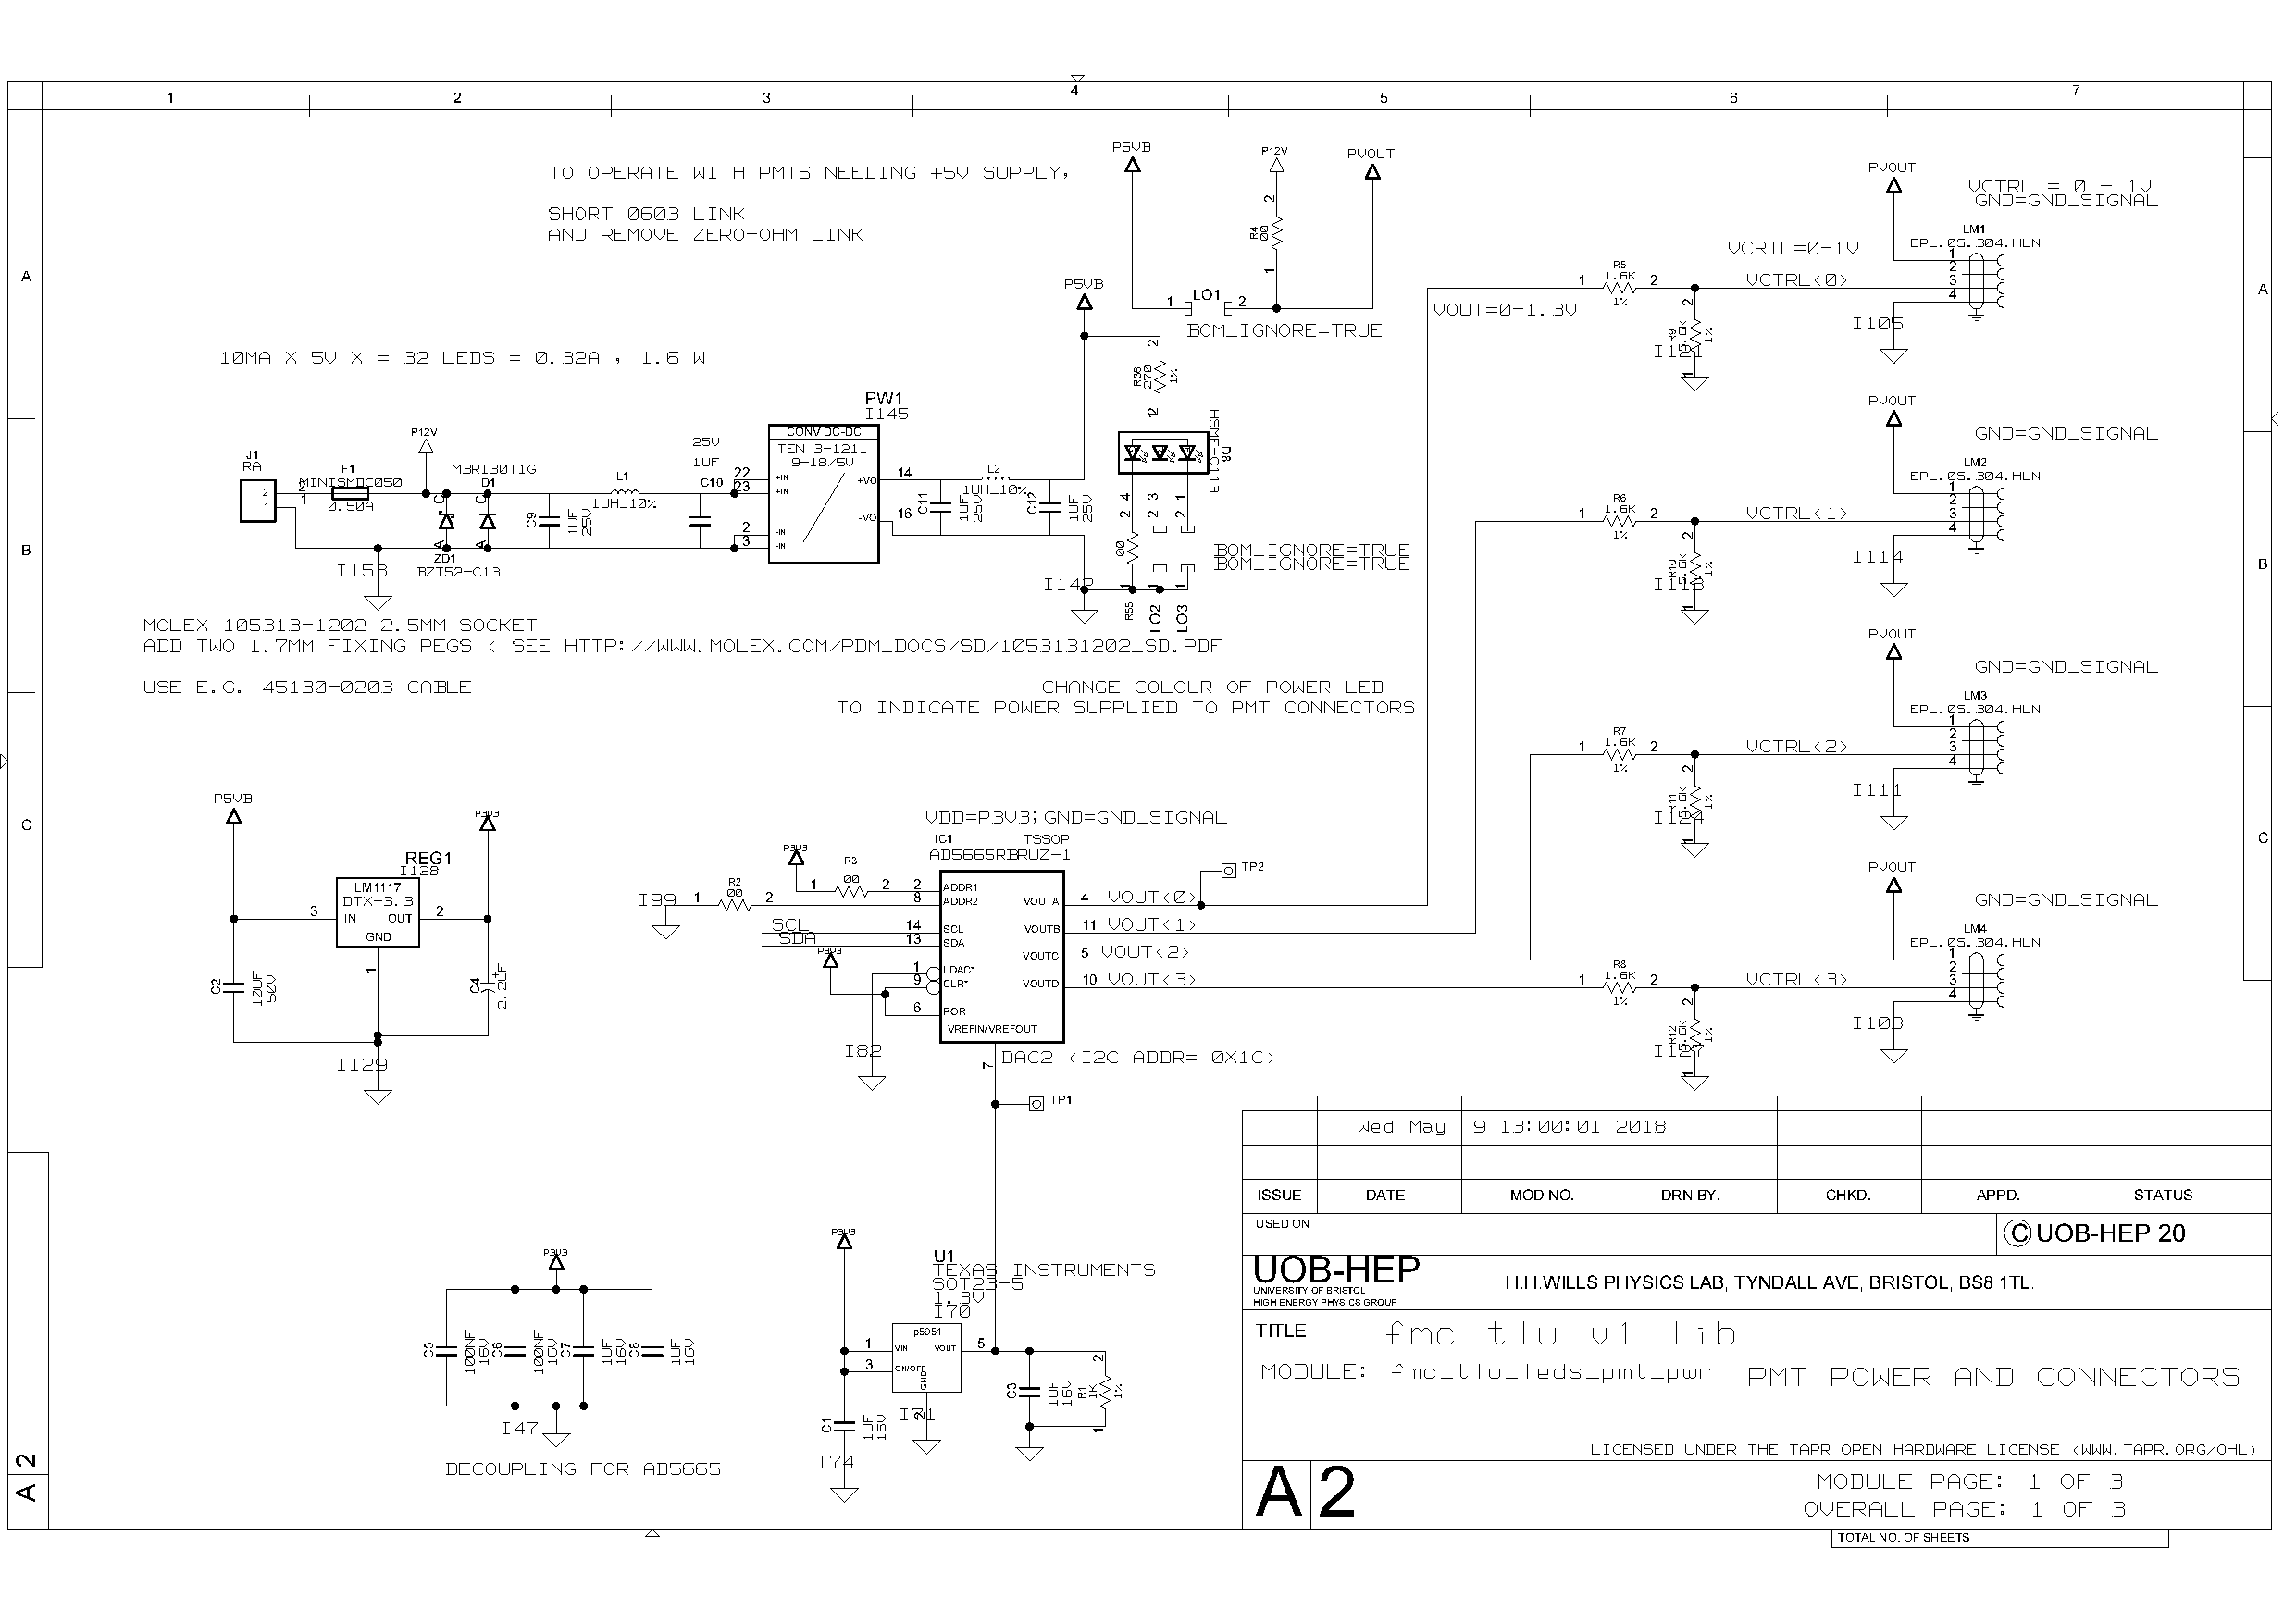
\includepdf[link,pages=-, angle=90]{./Docs/schematicsLED.pdf} 

%\begin{figure}[h]
%  \centering
%  \includegraphics[width=1.62\textwidth, angle=90]{./Images/protoDUNE_fmc_sfp_to_slave_v0-7.pdf}
%  \caption{Sketch of the connections and signal names between the elements of the board.}\label{fig:Connections}
%\end{figure}

%\section{Schematic}
%\includepdf[pages={1-},scale=0.99, landscape=true]{./Images/PC053A.pdf}
%%\includepdf[pages={1-},scale=0.99, landscape=true]{./Images/PC053A_TOPLEVEL.pdf}


%%% GLOSSARY
\printglossaries
%\printglossary[type=\acronymtype]
\printglossary[type=\acronymtype,title=Abbreviations]

%%% BIBLIOGRAPHY
%\bibliographystyle{unsrt}
%\bibliography{./../../Bibliography/myBibliography}


\end{document} 